
%%%%%%%%%%%%%%%%%%%%%%%%%%%%%%%%%%%%%%%%%%%%%%%%%%%%%%%%%%%%
%%%%%%%%%%%%%%%%%%%%%%%%%%%%%%%%%%%%%%%%%%%%%%%%%%%%%%%%%%%%%
%
%  %%%%%%%  %    %  %%%%%%  %%%%%%  %%%%%%%  %%%%%%%  %%%%%
%  %        %    %  %    %  %     %    %     %        %    %
%  %        %    %  %%%%%%  %     %    %     %        %    %
%  %        %%%%%%  %    %  %%%%%%     %     %%%%%    %%%%%
%  %        %    %  %    %  %          %     %        %    %
%  %%%%%%%  %    %  %    %  %          %     %%%%%%%  %     %
%
%%%%%%%%%%%%%%%%%%%%%%%%%%%%%%%%%%%%%%%%%%%%%%%%%%%%%%%%%%%%%
%%%%%%%%%%%%%%%%%%%%%%%%%%%%%%%%%%%%%%%%%%%%%%%%%%%%%%%%%%%%%

\chapter{The Definable Entrance Path Category}
\label{subsec:strat}

\begin{quote}
{\em ``Facilis descensus Averno;\\
noctes atque dies patet atri ianua Ditis;\\
sed revocare gradum superasque evadere ad auras,
hoc opus, hic labor est.''}
\begin{flushright} --- Virgil's Aeneid, Book 6, Lines 124-9 \end{flushright}
\end{quote}

Fundamentally, one-dimensional persistent homology tries to understand topological changes in a one-parameter family of spaces. Multi-dimensional persistence tries to understand topological changes in a multi-parameter family of spaces; the leap in complexity from one dimension to two can not be overstated. The model problem of interest is to describe how the homology of the fiber of a map $f:Y\to X$ changes as one queries points or subsets in $X$. For general maps, this problem is entirely too unwieldy. 

In this chapter we focus on a broad class of maps where this problem has an interesting answer: definably stratified maps. Informally, stratified maps are glued together fiber bundles. Definable maps are ones that can be defined with finitely many logical operations. Every definable map is stratified so we study simply definable maps.

The upshot of this chapter is that the homology of the fibers of a definable map give rise to a representation of a particular quiver with relations --- a category in other words --- called the definable entrance path category, whose general version was introduced by MacPherson to study general stratified maps. If one considers the opposite of the entrance path category, i.e. the exit path category, one obtains a constructible sheaf, which we now define.

\begin{defn}[Constructible Sheaves and Cosheaves]\index{sheaf!constructible}\index{sheaf!restricted sheaf}\index{cosheaf!constructible}
	Let $F$ be a sheaf valued on a topological space $X$. One says that $F$ is \textbf{constructible} if there exists a filtration by closed subsets $$\emptyset=X_{-1}\subset X_0 \subset X_1 \subset \cdots \subset X_n=X$$ 
	such that on the each connected component of the space $X^k=X_k- X_{k-1}$, the restricted sheaf $F|_{X^k}$ (the pullback of $F$ along the inclusion $X^k\hookrightarrow X$) is locally constant. Alternatively, instead of asking for a filtration one can ask for a decomposition of $X$ into disjoint pieces $X_{\sigma}$ over which the restricted sheaf is locally constant.

	Dually, we will call a cosheaf, with costalks valued in $\vect$, constructible if its linear dual is a constructible sheaf.
\end{defn}

One of the purposes of this chapter is to impose further conditions on the nature of the filtration so that we get nice properties. As stated, there is nothing to prevent us from using a one step filtration of the Cantor set. Expressing precisely these extra conditions will require the introduction of stratification theory.

\section{Stratification Theory and Tame Topology}
\label{subsec:strat_thy_tame_topology}

As wonderful as fiber bundles and local systems may be, they still fail to capture the sort of structure we are interested in because the topology of the fiber can never change. In order to bring cosheaves into contact into a larger realm of mathematics, we will need to consider stratified maps. To whet the appetite, stratified maps will allow us to describe in one language:
\begin{description}
	\item[Morse theory] --- Morse functions are just particular instances of stratified maps $f:M\to \RR$.
	\item[Picard-Lefschetz theory] --- the complex analog of Morse theory studies algebraic maps $\pi:X\to\CC$, which are necessarily stratified.
	\item[Point Cloud Data and Persistence] --- Semialgebraic families are described by semialgebraic maps, which are stratified.
\end{description}
In other words, stratification theory gives a system of geometry for exploring a wealth of examples, appearing in mathematics and nature. Stratification theory does this by breaking up a space or map into regions, over which the usual analysis of manifolds and fiber bundles apply.

\begin{defn}[Decomposition]\index{decomposition!into strata}\index{strata}
	A \textbf{decomposition} of a space $X$ is a locally finite partition of $X$ into locally closed subsets (sets of the form $U\cap Z$ for $U$ open and $Z$ closed) $\{X_{\sigma}\}_{\sigma\in P_X}$ called \textbf{pieces}, which satisfy the axiom of the frontier. Consequently, $P_X$ is a poset. When the pieces have the additional structure of being manifolds, we call them \textbf{strata}.
\end{defn}

\begin{rmk}
	A \textbf{stratum} is sometimes used to mean either a union of strata of a fixed dimension or a single connected component in a decomposition. We usually prefer the latter meaning.
\end{rmk}

We have already encountered an example of a decomposition of a space $X$, namely a cell complex. Here each piece is homeomorphic to $\RR^k$ for some $k$, which can vary from stratum to stratum. A graph is naturally decomposed into its vertices and open edges. For a decomposition that is not a cell complex, consider the complex numbers $\CC$ partitioned into the sets $\{0\}$ and $\CC-\,\{0\}$.

\begin{defn}
	Suppose $(X,P_X)$ and $(Y,P_Y)$ are decomposed spaces, then a \textbf{decomposition-preserving} map is a continuous map $f:X\to Y$ that sends pieces to pieces, i.e. we have a commutative square
	\[
	\xymatrix{X \ar[r]^f \ar[d] & Y \ar[d] \\ P_X \ar[r]^{P_f} & P_Y}
	\]
	In the case where the pieces are strata we call such a map a \textbf{stratum-preserving} map.
\end{defn}

Much like how the notion of a category emerged through the study of functors, in some sense the necessity for decompositions more general then simplicial or cell complexes came about because not all maps preserved the pieces of those decompositions. We give an example of such a map.

\begin{ex}[Blow-Ups]\label{ex:blowup}\index{blow-up}
	Consider the map
	\[
		f:\RR^2\to\RR^2 \qquad f(x,y)=(x,xy).
	\]
	This map is not triangulable, see~\cite{shiota} page 305. This map is related to the operation in algebraic geometry known as ``blowing up at a point.'' The blow-up map is an endless source of interesting geometry and counter-examples, so it is worth describing. Recall that the space of lines in $\RR^2$, written $\RR\mathbb{P}^1$ is defined to be the quotient of $\RR^2-\,\{(0,0)\}$ by the relation that $(x,y)\sim (\lambda x,\lambda y)$ for any $\lambda\neq 0$. Topologically, this quotient is the circle $S^1$. Tracing the image of the top arc of a circle from $0$ to $\pi$ through the quotient map one gets the complete circle in $\RR\mathbb{P}^1$.
	
	The blow-up $B$ of $\RR^2$ at the origin is defined to be the closure of the image of the map
	\[
		\RR^2-\,\{(0,0)\} \hookrightarrow \RR^2\times \RR\mathbb{P}^1
	\]
	where the map to the first coordinate is the inclusion and the map to the second coordinate is the quotient map. The blow-up map $\pi:B\to\RR^2$ is the projection back from the closure of the graph of this map to the closure of the domain, i.e. $\RR^2$. Thus the fiber over $(0,0)$ is a circle, but the fiber over any other point is a single point. One can visualize this by restricting the map to a closed disk centered at the origin. The image is contained in a solid torus and the closure of the image will assign the core circle to the origin. The image of $\mathbb{D}^2-\,\{(0,0)\}$ is commonly visualized as a spiral staircase as in Figure~\ref{fig:blowup} whose boundary traces out a torus knot. See \cite{arone-blowup} for a treatment of different constructions of real blow-ups and their functorial properties.
\end{ex}

\begin{figure}
\centering
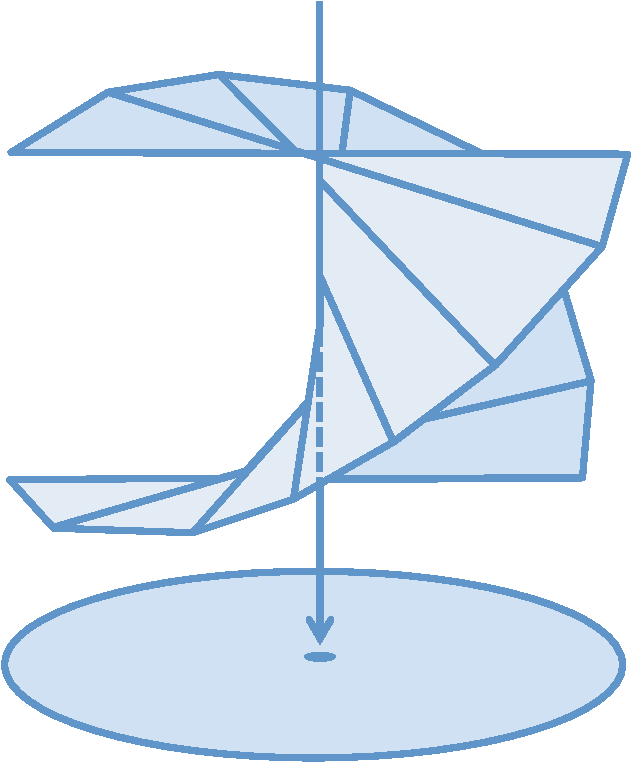
\includegraphics[width=.7\textwidth]{blowup_closed_disc.pdf}
\caption{Blowing up at a Point}
\label{fig:blowup}
\end{figure}


\begin{figure}
\centering
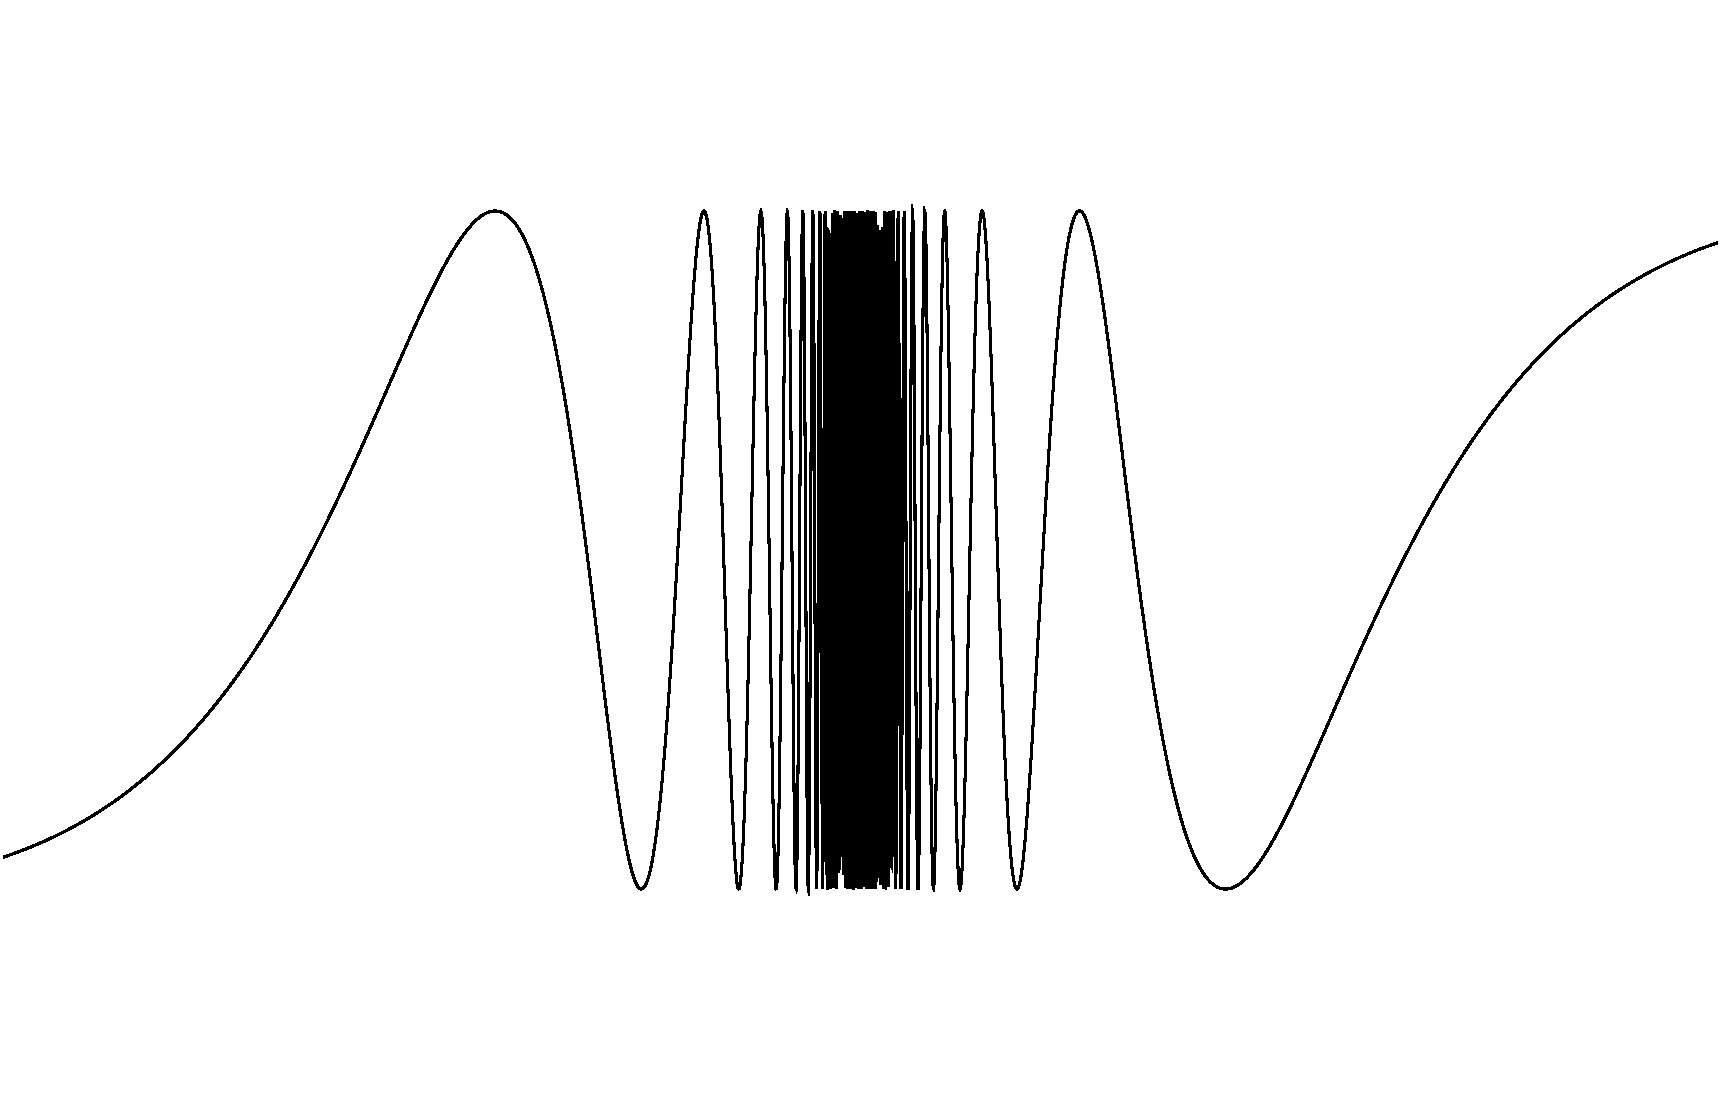
\includegraphics[width=.5\textwidth]{top_sine.pdf}
\caption{Topologist's Sine Curve}
\label{fig:top_sine}
\end{figure}

Decomposing spaces and maps gives some control over how these things are built up out of pieces, but it is not quite strong enough to tame the geometry of interest. In particular, the topologist's sine curve drawn in Figure \ref{fig:top_sine} can be decomposed into the two pieces
\[
	X_{\tau}:=\{(x,\sin(1/x))\, |\, x\neq 0 \}\cup \{(0,y)\,|\, y\in[-1,1]\}=:X_{\sigma}
\]
that satisfy the axiom of the frontier $X_{\sigma}\subset \bar{X}_{\tau}$, but it does not have the intuitively desired property that~\cite[p.131]{lu-ctst}.
\[
	\dim X_{\sigma} < \dim X_{\tau}
\]


Further regularity conditions must be imposed to capture this property and other desired features that hold for piecewise-linear, algebraic, semi-algebraic, sub-analytic and other geometries. Systematic overviews of these different regularity conditions are overwhelming and highly technical. For a taste, one should consult J\"org Sch\"urmann's remarkable service in writing down 14 different regularity conditions and their corresponding implications in~\cite[Rmk. 4.1.9]{schurmann}. To keep the exposition light we focus on a geometric condition and its topological generalization as they have historically had a strong influence on stratification theory.

\subsection{Whitney Stratified Spaces}
\label{subsubsec:whitney}

In this section we relay two ways of fusing manifold pieces into non-manifold wholes. The champions of this section are Hassler Whitney and Ren\'e Thom.\footnote{For more historical context of these approaches, written by experts, we recommend the recent article~\cite{goresky-bull} and Part I, Section 1 of~\cite{GM}.} In 1965, Whitney, whose approach relies on the geometry of tangent planes and secant lines, defined two properties that a stratified space should possess~\cite{whitney-local, whitney1965annals}. Thom, who proposed in a 1962 paper~\cite{thom-poly} a definition of a stratified space using tubular neighborhoods, later extracted the topological consequences of Whitney's definition and outlined a more general definition of a stratified space~\cite{thom-strat}. Thom's definition was first articulated carefully by John Mather in his famous 1970 Harvard ``Notes on Topological Stability''~\cite{mather}, which went unpublished for 42 years and are to this day an excellent resource for learning the theory. 

Proving that any Whitney stratified space admits the structure of a Thom-Mather stratified space requires substantial work. Thus, we present them below as separate definitions, beginning with Whitney's. We outline the properties that make Whitney stratified spaces nice as motivation for Thom's definition. After introducing both of these definitions we will present a proof\footnote{A proof appears in Mark Goresky's thesis~\cite{goresky-thesis} that was never published and which he graciously provided to the author. We have since modified that proof to suit our purposes.} that says that closed unions of strata in a Thom-Mather space have regular neighborhoods, i.e. an open neighborhood and a weak deformation retraction. This result plays a key role in Theorem \ref{thm:strat_maps}.

\begin{figure}
	\centering
	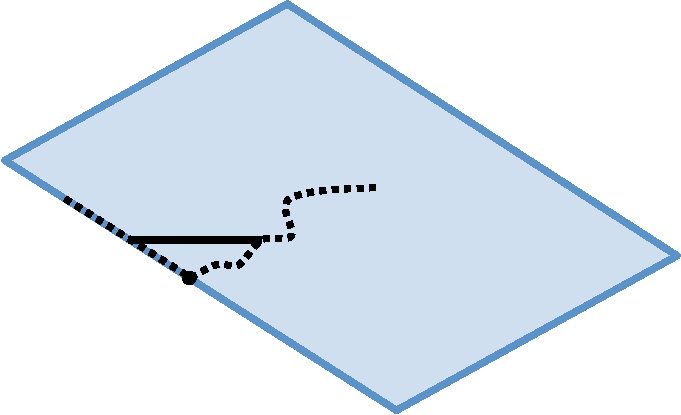
\includegraphics[width=.6\textwidth]{whitney_b_bold.pdf}
	\caption{Diagram for Whitney Condition (b)}
	\label{fig:whitney_b}
\end{figure}

\begin{defn}[Whitney Stratified Spaces]\index{stratified space!Whitney}
	A \textbf{Whitney stratified space} is a tuple $(X,M,\{X_{\sigma}\}_{\sigma\in P_X})$ where $X$ is a closed subset of a smooth manifold $M$ along with a decomposition into pieces $\{X_{\sigma}\}_{\sigma\in P_X}$ such that
	\begin{itemize}
		\item each piece $X_{\sigma}$ is a locally closed smooth submanifold of $M$, and
		\item whenever $X_{\sigma}\leq X_{\tau}$ the pair satisfies \textbf{condition (b)}. This condition says if $\{y_i\}$ is a sequence in $X_{\tau}$ and $\{x_i\}$ is a sequence in $X_{\sigma}$ converging to $p\in X_{\sigma}$ and the tangent spaces $T_{y_i}X_{\tau}$ converges to some plane $T$ at $p$, and the secant lines $\ell_i$ connecting $x_i$ and $y_i$ converge to some line $\ell$ at $p$, then $\ell\subseteq T$.
	\end{itemize}
\end{defn}
\begin{rmk}
	We have omitted \textbf{condition (a)} because it is implied by condition (b)~\cite[Prop. 2.4]{mather}. Condition (a) states that if we only consider a sequence $y_i$ in $X_{\tau}$ converging to $p$ such that the tangent planes $T_{y_i}X_{\tau}$ converge to some plane $T$, then the tangent plane to $p$ in $X_{\sigma}$ must be contained inside $T$.
\end{rmk}

The Whitney conditions are important because so many types of spaces admit Whitney stratifications, the most important being semi-algebraic and sub-analytic spaces.  Remarkably, these conditions about limits of tangent spaces and secant lines imply strong structural properties of the space. To give the reader a taste for the properties enjoyed by Whitney stratified spaces, we provide a brief list:\footnote{Here we follow part of MacPherson's summary in the appendix of his 1991 Colloquium notes~\cite{macpherson-ih-notes}.}
\begin{itemize}\index{stratified space!general properties of}
	\item[-] \textbf{Dimension is Well-Behaved:} If $X_{\sigma}\subseteq \fr(X_{\tau}):=\bar{X}_{\tau}-X_{\tau}$, then $\dim X_{\sigma} < \dim X_{\tau}$. See Proposition 2.7 of~\cite{mather} for a proof. This rules out the topologist's sine curve in Figure \ref{fig:top_sine} from being Whitney stratified.
	\item[-] \textbf{Good Group of Self-Homeomorphisms:} If $x$ and $y$ belong to the same connected component of a stratum $X_{\sigma}$, then there is a homeomorphism $h:M\to M$ preserving $X$ and other strata such that $h(x)=y$ (\cite{mather} pp. 480-481).
	\item[-] \textbf{Local Bundle Structure:} Every stratum $X_{\sigma}$ has an open tubular neighborhood $T_{\sigma}$ and a projection map $\pi_{\sigma}:T_{\sigma}\to X_{\sigma}$ making it into a fiber bundle. This bundle is equipped with a ``distance from the stratum'' function $d_{\sigma}:T_{\sigma}\to\RR_{\geq 0}$. If we define $S_{\sigma}(\epsilon)$ to be $d^{-1}_{\sigma}(\epsilon)$, then we can identify the map $\pi_{\sigma}:T_{\sigma}\to X_{\sigma}$ with the mapping cylinder of the restricted map $\pi:S_{\sigma}(\epsilon)\to X_{\sigma}$ (\cite{goresky-fol} p. 194). Moreover, the fiber of the bundle has the stratification of a cone on a link.
	\item[-] \textbf{Triangulability:} Every Whitney stratified space can be triangulated~\cite{goresky-fol}.
\end{itemize} 

The third property is historically the most important. It guarantees that a Whitney stratification ``looks the same'' along all points in a stratum. The tubular neighborhoods exhibit this local triviality. This condition will be taken as primary when considering Thom-Mather stratifications.

\subsection{Stratified Maps and a Counterexample}
\label{subsubsec:strat_maps}

Our main purpose for considering Whitney (and hence Thom-Mather) stratified spaces is to understand stratified maps. Such maps include Morse functions as a special case and are a good model for understanding moduli problems that commonly arise in applications. Over a given stratum, a stratified map looks like a fiber bundle and all fibers are homeomorphic in a stratum-preserving way. However, as we try to compare a fiber over one stratum with a fiber over that stratum's frontier, the blow-up map of Example \ref{ex:blowup} frustrates our intuition. Thus, we introduce a more restrictive class of stratified maps called Thom maps. Finally, we illustrate that such general stratified maps are not necessarily closed under pullback. This motivates the move to tame topology in Section \ref{subsubsec:tame_topology}.

\begin{defn}[Whitney Stratified Map]\index{stratified map!Whitney}
	Suppose $f:M\to N$ is a smooth map between manifolds that contain stratified spaces $(X,\{X_{\sigma}\}_{\sigma\in P_X})$ and $(Y,\{Y_{\sigma}\}_{\sigma\in P_Y})$ such that $f(X)\subset Y$ with $f|_X$ \emph{proper}. We say $f$ is a Whitney \textbf{stratified map} if the pre-image of each stratum $Y_{\sigma}$ is a union of connected components of strata of $X$ and $f$ takes these components submersively onto $Y_{\sigma}$.
\end{defn}
\begin{rmk}
	To say that a map is (Whitney) \textbf{stratifiable} is to say there exists a stratification of $X$ and $Y$ such that the map is stratified. Often we will neglect to include the ambient manifolds and will say ``Let $f:X\to Y$ be a stratified map.'' 
\end{rmk}
\begin{rmk}\index{stratified submersion}
	When $N=Y$ is stratified as a single stratum, we say that $f$ is a \textbf{stratified submersion}, i.e. $f|_X$ is proper and for each stratum $X_{\sigma}$ $f|_{X_{\sigma}}$ is a submersion.
\end{rmk}

Recall that Ehresmann's theorem states that proper submersions are fiber bundles. Thus, over each stratum a stratified map is a fiber bundle. However, Ehresmann's theorem does not say that the local trivializations can be chosen to respect the stratification. This stratified analog of Ehresmann's theorem is expressed in Thom's first isotopy lemma~\cite[p.~41]{GM}.

\begin{lem}[Thom's First Isotopy Lemma]\label{lem:thom_1}\index{Thom's first isotopy lemma}
	Let $f:M\to \RR^n$ be a (proper) stratified submersion for $X\subseteq M$ a Whitney stratified subset. Then there is a stratum-preserving homeomorphism
	\[
	h: X \to \RR^n\times (f^{-1}(0)\cap X)
	\]
	which is smooth on each stratum and commutes with the projection to $\RR^n$. In particular, the fibers of $f|_X$ are homeomorphic by a stratum preserving homeomorphism.
\end{lem}
\begin{rmk}
	Of course, this implies that for a general stratified map, for every stratum of the codomain $Y_{\sigma}$, the fibers of $f|_{f^{-1}(Y_{\sigma})}:f^{-1}(Y_{\sigma}) \to Y_{\sigma}$ are homeomorphic in a stratum-preserving way. This lemma will be used implicitly throughout the section. It expresses the idea that stratified maps are ``glued together fiber bundles.''
\end{rmk}

As one can imagine, there is a second isotopy lemma, which applies to a more restrictive class of stratified maps. We will not state the second isotopy lemma, rather we will use some of the theory leading up to it.

\subsubsection{Counterexamples Creep In}

One would like to say that given a general (not necessarily Thom) stratified map $f:X\to Y$, one could take a path $\gamma:[0,1]\to Y$ so that the pullback $\gamma^* f:f^{-1}(\gamma)\to I$ is stratified and hence, by the above corollary, a Thom mapping. However, as the next example shows, the pullback need not be stratifiable, so the hypothesis for the corollary fails.\footnote{We are indebted to Mark Goresky for suggesting the key ideas of this example.}

\begin{figure}
\centering
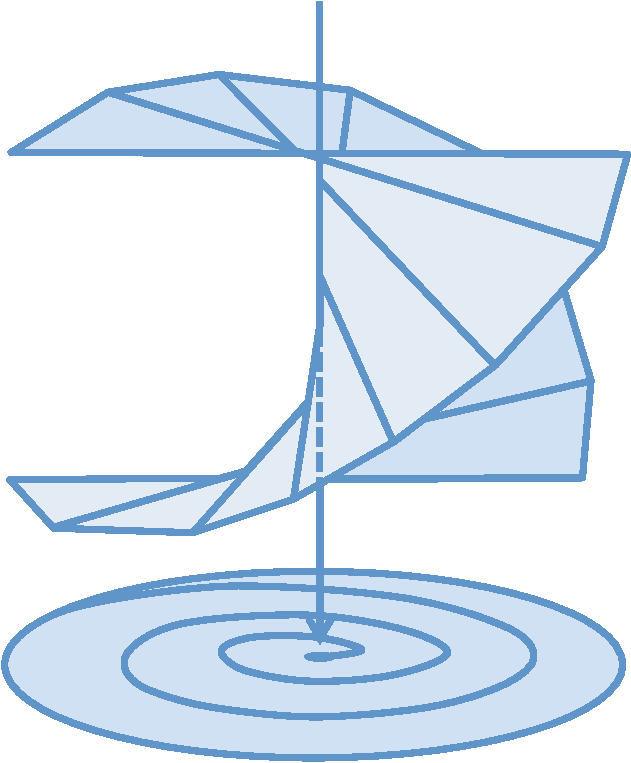
\includegraphics[width=.7\textwidth]{blowup_spiral.pdf}
\caption{Preimage of the Spiral is Not Stratifiable}
\label{fig:blowup_cex}
\end{figure}

\begin{ex}\label{ex:pullback_spiral}
	The blow-up map $\pi:B\to\RR^2$ is a Whitney stratified map that is not a Thom mapping. The closure $S$ of the ``quick spiral''
	\[
		S:=\mathrm{cl}\{(r,\theta)\in\RR^2 \,|\, r=e^{-\theta^2}\}
	\]
	is also Whitney stratified despite wrapping around the origin infinitely many times (\cite{pflaum} Example 1.4.8). However, the inverse image $\pi^{-1}(S)$ cannot be stratified because the inverse image of $(0,0)$ is $S^1$, which is of the same dimension as the inverse image of the spiral, despite the fact that the former is in the frontier of the latter; see Figure~\ref{fig:blowup_cex}. Since being Whitney stratified implies a drop in dimension of the frontier, contraposition shows that the inverse image cannot be Whitney stratified.
\end{ex}

In Theorem \ref{thm:strat_maps} we will give a direct geometric construction of several cosheaves associated to a stratified map. To do so we will need to consider a class of subsets and maps that have all the geometric properties of stratified spaces as well as being preserved under inverse images. This is provided in Section \ref{subsubsec:tame_topology}.

\subsection{O-minimal Structures}
\label{subsubsec:tame_topology}\index{tame topology}

Although stratification theory provides a first pass at taming geometry, it is unsuitable from our perspective because pathologies can still creep in via the inverse image, as Example \ref{ex:pullback_spiral} showed. General stratified spaces and maps are still not tame enough. However, most sets and maps encountered in nature have extra structure. For instance, computer scientists commonly work with piecewise-linear (PL) spaces, which are describable in terms of affine spaces and matrix inequalities. Some algebraic geometers work with semialgebraic spaces, which use zeros and inequalities of polynomials to define their spaces. Analysts tend to use analytic or subanalytic spaces, because the theory is well behaved. Traditionally, one has had to make a choice, once and for all, to speak only of PL geometry, or only of algebraic geometry, or only of analytic geometry. The curse of Babel has confused and separated these domains for a hundred years.

In 1984, Grothendieck declared that an axiomatic ``tame topology'' or ``topologie mod\'er\'ee'' should be developed by extracting out precisely those properties that make these classes of spaces good ones~\cite{grothendieck-sketch}. MacPherson put forth in his lecture notes for the 1991 AMS colloquium lectures a definition of what should constitute a ``good'' class of subsets of a manifold $M$~\cite{macpherson-ih-notes}. Namely, a subset $S$ is good if there is a Whitney stratification of $M$ such that $S$ is a union of strata. These subsets should be closed under the finite set-theoretic operations of unions, intersections and differences. Additionally, the closure of any good subset should be good.

In 1996, Lou van den Dries and his student Chris Miller set forth a most satisfactory definition in their paper ``Geometric Categories and O-minimal Structures''~\cite{vdd-geocat}. Taking requests from sheaf theorists~\cite{schmid-cc} and other working geometers, their paper is a valuable service to the community. It globalized a local solution to Grothendieck's program known as \textbf{o-minimal topology}. The theory of o-minimal topology is grounded in model theory and logic, but it has left almost no trace from those fields. All the logical operations of $\forall,\exists,\lor,\land$ are converted into familiar operations in geometry. Each of the above languages (PL, semialgebraic, subanalytic) are instances of an o-minimal structure. The common fundamental theorems, each expressed in their own language, can be reduced to universal logical operations, and hence geometric ones. We will start by examining o-minimal structures as they form the local models of Miller and van den Dries definition. The reader is urged to consult the textbook ``Tame Topology and O-minimal Structures''~\cite{vdd-ttos} as it is an excellent introduction that requires virtually no pre-requisites.

\begin{defn}[\cite{vdd-ttos}, p. 2]\index{o-minimal structure}
 An \textbf{o-minimal structure on $\RR$} is a sequence $\OO=\{\OO_n\}_{n\geq 0}$ satisfying
 \begin{enumerate}
  \item $\OO_n$ is a boolean algebra of subsets of $\RR^n$, i.e. it is a collection of subsets of $\RR^n$ closed under unions and complements, with $\emptyset \in\OO_n$;
  \item If $A\in\OO_n$ then $A\times\RR$ and $\RR\times A$ are both in $\OO_{n+1}$;
  \item The sets $\{(x_1,\ldots,x_n)\in\RR^n|x_i=x_j\}$ for varying $i\leq j$ are in $\OO_n$;
  \item If $A\in\OO_{n+1}$ then $\pi(A)\in\OO_{n}$ where $\pi:\RR^{n+1}\to\RR^n$ is projection onto the first $n$ factors;
  \item For each $x\in\RR$ we require $\{x\}\in\OO_1$ and $\{(x,y)\in\RR^2|x<y\}\in\OO_2$;
  \item The only sets in $\OO_1$ are the finite unions of open intervals and points.
 \end{enumerate}
When working with a fixed o-minimal structure $\OO$ on $\RR$ we say a subset of $\RR^n$ is \textbf{definable} if it belongs to $\OO_n$. A map is definable if its graph is definable.
\end{defn}

\begin{rmk}
	One should note that the third and sixth property together prohibit any spiral that wraps infinitely many times around the origin from being part of an o-minimal structure. Thus, the quick spiral in Example \ref{ex:pullback_spiral} is not definable.
\end{rmk}

Now we prove that definable sets and maps are closed under pullbacks.
\begin{lem}\label{lem:def_pb}
Suppose $f:X\to Z$ and $g:Y\to Z$ are definable maps, then the pullback $X\times_Z Y:=\{(x,y)\in X\times Y\,|\, f(x)=g(y)\}$ is a definable set and the restrictions of the projection maps are definable as well.
\end{lem}
\begin{proof}
 First note that if $X\in \OO_n$ and $Y\in \OO_m$, then $X\times Y=(X\times \RR^m)\cap (\RR^n\times Y)$ is in $\OO_{n+m}$. Since $\Gamma_f$ and $\Gamma_g$ are definable, we know that $\Gamma_f\times Y=\{(x,y,f(x))\}$ and $\Gamma_g\times X=\{(x',y',g(y')\}$ are both definable subsets of $X\times Y\times Z$. Since the intersection is definable, and a point in the intersection has $(x,y,f(x))=(x',y',g(y'))$, the image of the projection to $X\times Y$ is the pullback. One can then use B.3 of~\cite{vdd-geocat} to conclude that the restriction to the pullback of the projection maps to $X$ and $Y$ is definable as well.
\end{proof}

There are surprising facts that follow from the axioms of an o-minimal structure. For example, if $A\in\OO$, then the closure $\bar{A}$ is in $\OO$ (\cite{vdd-ttos} Ch. 1, 3.4). Another surprising fact is that definable sets can be Whitney stratified~\cite{loi-verdier}. Thus, these sets meet the requirements of MacPherson to form a good class of subsets. Perhaps even better than MacPherson's sets, definable sets can be given finite cell decompositions, where ``cell'' has its own special meaning (\cite{vdd-ttos} Ch. 3).

The prototypical o-minimal structure is the class of semialgebraic sets, which has become increasingly relevant in applied mathematics.

\begin{defn}\index{semialgebraic subset}
	A \textbf{semialgebraic} subset of $\RR^n$ is a subset of the form
	\[
		X=\bigcup_{i=1}^p\bigcap_{j=1}^q X_{ij}
	\]
	where the sets $X_{ij}$ are of the form $\{f_{ij}(x)=0\}$ or $\{f_{ij}>0\}$ with $f_{ij}$ a polynomial in $n$ variables.
\end{defn}

	The only semi-algebraic subsets of $\RR$ are finite unions of points and open intervals. From the definition, one sees that the class of semialgebraic sets is closed under finite unions and complements. The \textbf{Tarski-Seidenberg} theorem states that the projection onto the first $m$ factors $\RR^{m+n}\to\RR^m$  sends semialgebraic subsets to semialgebraic subsets~\cite{coste-sag}. We can deduce from this theorem all of the conditions of o-minimality.
	
	Semialgebraic maps are defined to be those maps $f:\RR^k\to \RR^n$ whose graphs are semialgebraic subsets of the product. It is a fact that semi-algebraic sets and maps can be Whitney stratified~\cite{shiota-geometry}. This allows us to consider the following example of a semi-algebraic family of sets:
	
	\begin{figure}
		\centering
		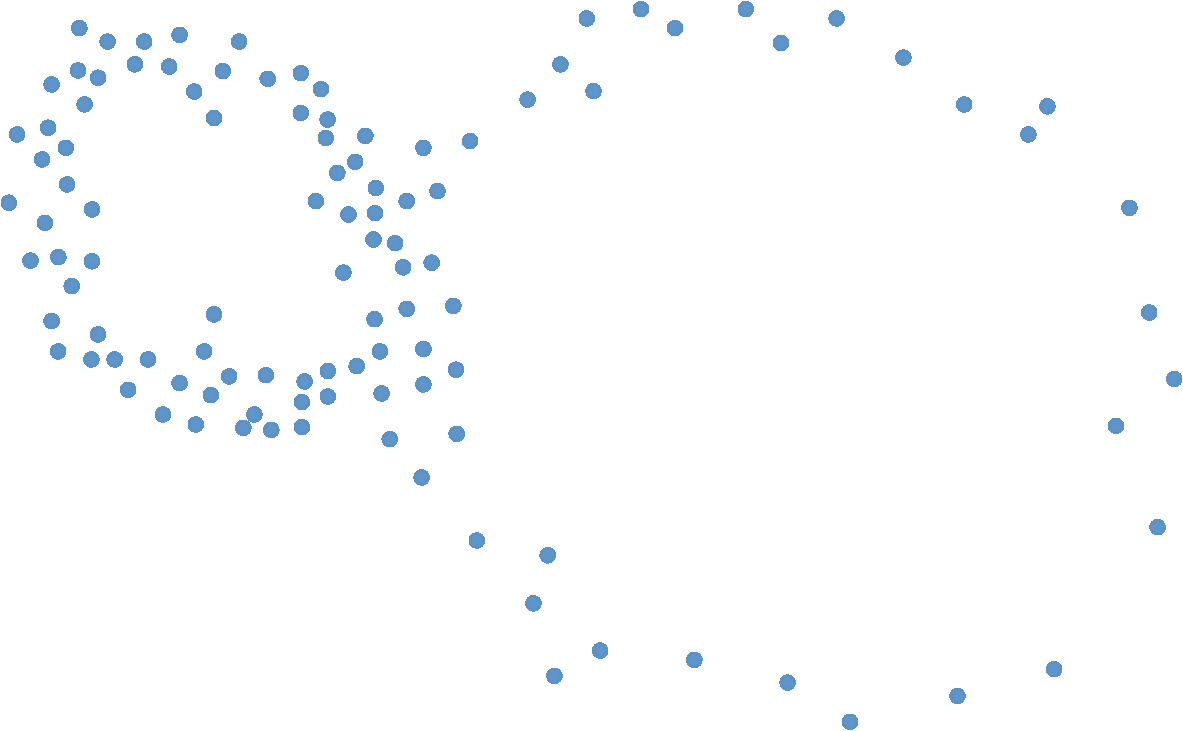
\includegraphics[width=.9\textwidth]{point_cloud2.pdf}
		\caption{Point Cloud Data}
		\label{fig:point_cloud}
	\end{figure}

\begin{ex}[Point-Cloud Data]\label{ex:pcd}\index{point cloud}
	Suppose $Z$ is a finite set of points in $\RR^n$. For each $z\in Z$, consider the square of the distance function
	\[f_z(x_1,\ldots,x_n)=\sum_{i=1}^n (x_i-z_i)^2.\]
	By the previously stated facts we know that the sets
	\[
		B_z:=\{x\in\RR^{n+1} \, | \, f_z(x_1,\ldots,x_n)\leq x_{n+1}\}
	\]
	are semialgebraic along with their unions and intersections. Denote by $X$ the union of the $B_z$. The Tarski-Seidenberg theorem implies that the map
	\[
		f:X\to\RR \qquad f^{-1}(r):=\cup_{z\in Z} B(z,\sqrt{r})=\{x\in\RR^n \, | \, \exists z\in Z \, \mathrm{s.t.} \, f_z(x)\leq r\}	\]
	is semialgebraic. In particular the topology of the fiber (of the union of the closed balls) can only change finitely many times.
\end{ex}

We conclude with the definition Miller and van den Dries proposed in section 1 of~\cite{vdd-geocat}. This definition allows us to verify definability locally, and allows us to work inside manifolds other than $\RR^n$.

\begin{defn}[Analytic-Geometric Categories]\index{analytic-geometric category}\index{o-minimal structure!analytic-geometric category}
	A \textbf{analytic-geometric category} $\calG$ is given by assigning to each analytic manifold $M$ a collection of subsets $\calG(M)$ such that following conditions are satisfied:
	\begin{enumerate}
		\item $\calG(M)$ is a boolean algebra of subsets of $M$, with $M\in\calG(M)$.
		\item If $A\in\calG(M)$, then $A\times\RR\in\calG(M)$.
		\item If $f:M\to N$ is a proper analytic map and $A\in\calG(M)$, then $f(A)\in\calG(N)$.
		\item If $A\subseteq M$ and $\{U_i\}_{i\in\Lambda}$ is an open covering of $M$, then $A\in\calG(M)$ if and only if $A\cap U_i\in\calG(U_i)$ for all $i\in\Lambda$.
		\item Every bounded set in $\calG(\RR)$ has finite boundary.
	\end{enumerate}
\end{defn}
\begin{rmk}
This defines a category in the usual sense. An object of $\calG$ is a pair $(A,M)$ with $A\in\calG(M)$. A morphism $f:(A,M)\to (B,N)$ is a continuous map $f:A\to B$ whose graph
\[
	\Gamma(f):=\{(a,f(a))\in M\times N\,|\, a\in A\}
\]
is an element of $\calG(M\times N)$.
\end{rmk}

The category of $\calG$-sets and $\calG$-maps, although we will prefer to use the term ``definable,'' has all the properties one could desire, including being closed under inverse images~\cite[D.7]{vdd-geocat} (as long as the domain is closed) and Whitney stratifiability~\cite[D.16]{vdd-geocat}.\footnote{The authors of~\cite{vdd-geocat} acknowledge that there is a gap in the proof of Whitney stratifiability of $\calG$-maps, but Ta L\^{e} Loi~\cite{loi-omin} and others~\cite{definably-stratified} have since filled in this gap.}


\subsection{Thom-Mather Stratifications}

\begin{defn}[Control Data]\index{control data}
	Let $(X,M,\{X_{\sigma}\}_{\sigma\in P_X})$ be a Whitney stratified space and $\{(T_{\sigma},\pi_{\sigma},d_{\sigma})\}$ a family of tubular neighborhoods. We call this family a system of \textbf{control data} if the following commutation relations are satisfied: if $X_{\sigma}\leq X_{\tau}$, then
	\begin{eqnarray*}
		\pi_{\sigma}\circ \pi_{\tau} &=& \pi_{\sigma} \\
		d_{\sigma}\circ \pi_{\tau}&=& d_{\sigma}
	\end{eqnarray*}
whenever both sides of the equations are defined.
\end{defn}

\begin{figure}
	\centering
	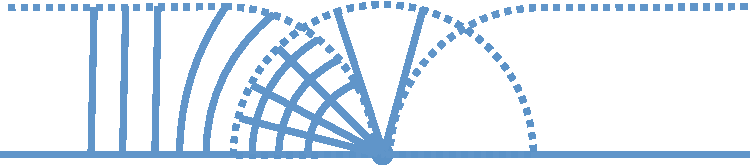
\includegraphics[width=.9\textwidth]{control.pdf}
	\caption{A System of Control Data}
	\label{fig:control}
\end{figure}
\begin{rmk}
In Figure~\ref{fig:control} we have drawn some fibers of the retraction maps for two incident strata. Notice how the fibers must bend in order for the second compatibility condition to hold.
\end{rmk}

Mather proves that every Whitney stratified space admits a system of control data. The following definition axiomatizes the properties enjoyed by a Whitney space with a system of control data.

\begin{defn}[Thom-Mather Stratified Spaces]\index{stratified space!Thom-Mather}
	A \textbf{Thom-Mather stratified space} consists of a Hausdorff, locally compact topological space $X$ with countable basis for its topology with some smooth structure; a decomposition into topological manifolds $\{X_{\sigma}\}_{\sigma\in P_X}$; and a family of control data $\{(T_{\sigma},\pi_{\sigma},d_{\sigma})\}_{\sigma\in P_X}$, where $T_{\sigma}$ is an open tubular neighborhood of $X_{\sigma}$, $\pi_{\sigma}:T_{\sigma}\to X_{\sigma}$ is a continuous retraction, and $d_{\sigma}:X_{\sigma}\to [0,\infty)$ is a continuous distance function. We require that the following conditions hold:
	\begin{itemize}
		\item $X_{\sigma}=d_{\sigma}^{-1}(0)$ for all $\sigma$.
		\item For any pair of strata $X_{\sigma}, X_{\tau}$, define $T_{\sigma,\tau}:=T_{\sigma}\cap X_{\tau}$, $\pi_{\sigma,\tau}:=\pi_{\sigma}|_{T_{\sigma,\tau}}$ and $d_{\sigma,\tau}:=d_{\sigma}|_{T_{\sigma,\tau}}$. We require that
		\[
			(\pi_{\sigma,\tau},d_{\sigma,\tau}): T_{\sigma,\tau}\to X_{\sigma}\times (0,\infty)
		\]
		is a smooth submersion. When $T_{\sigma,\tau}\neq\emptyset$, i.e. when $X_{\sigma}\leq X_{\tau}$, this implies $\dim X_{\sigma} < \dim X_{\tau}$.
		\item For any trio of strata $X_{\sigma}, X_{\tau}$ and $X_{\lambda}$ we have
		\begin{eqnarray*}
			\pi_{\sigma,\tau}\circ \pi_{\tau,\lambda}&=&\pi_{\sigma,\lambda} \\
			d_{\sigma,\tau}\circ \pi_{\tau,\lambda}&=& d_{\sigma,\lambda}
		\end{eqnarray*}
		whenever both sides of the equation are defined.
	\end{itemize}
\end{defn}
\begin{rmk}
	One should observe that the definition does not require an embedding into an ambient space. Thus Thom-Mather stratified spaces allow us to treat Whitney stratified spaces intrinsically. Any Whitney stratified space $(X,M)$ equipped with a system of control data $\{(T_{\sigma},\pi_{\sigma},d_{\sigma})\}_{\sigma\in P_X}$ defines a Thom-Mather stratified space by intersecting each $T_{\sigma}$, which is open in $M$, with $X$.
\end{rmk}

Thom-Mather stratified spaces exhibit most of the good properties of Whitney stratified spaces. The proof that Thom-Mather spaces can be triangulated was carried out by Goresky~\cite{goresky-fol}, among others. His proof views the lines of Figure \ref{fig:control} not as fibers of the retraction map $\pi_{\sigma}$, but rather\footnote{This description does not hold in higher dimensions.} as fibers of a radial projection map to the boundary of a tubular neighborhood.

\begin{defn}[Family of Lines]\label{defn:fol}\index{family of lines}
	A \textbf{family of lines} on a Thom-Mather stratified space is a system of radial projections
\[
	r_{\sigma}(\epsilon):T_{\sigma}-X_{\sigma}\to S_{\sigma}(\epsilon):=d_{\sigma}^{-1}(\epsilon)
\]
one for each stratum $X_{\sigma}$, and a positive number $\delta$, such that whenever $0<\epsilon <\delta$ and $X_{\sigma}\leq X_{\tau}$, the following commutation relations hold:
\begin{enumerate}
	\item $r_{\sigma}(\epsilon)\circ r_{\tau}(\epsilon')=r_{\tau}(\epsilon')\circ r_{\sigma}(\epsilon)\in S_{\sigma}(\epsilon)\cap S_{\tau}(\epsilon')$
	\item $d_{\sigma}\circ r_{\tau}(\epsilon)=d_{\sigma}$
	\item $d_{\tau}\circ r_{\sigma}(\epsilon)=d_{\tau}$
	\item $\pi_{\sigma}\circ r_{\tau}(\epsilon)=\pi_{\sigma}$
	\item If $0<\epsilon <\epsilon'<\delta$, then $r_{\sigma}(\epsilon')\circ r_{\sigma}(\epsilon)=r_{\sigma}(\epsilon')$
	\item $\pi_{\sigma}\circ r_{\sigma}(\epsilon)=\pi_{\sigma}$
	\item $r_{\sigma}(\epsilon)|_{T_{\sigma}(\epsilon)\cap X_{\tau}}:T_{\sigma}(\epsilon)\cap X_{\tau}\to S_{\sigma}(\epsilon)\cap X_{\tau}$ is smooth
\end{enumerate}
\end{defn}
\begin{rmk}
Every Thom-Mather stratified space admits a family of lines. This is the first proposition of~\cite{goresky-fol}.
\end{rmk}

Any family of lines can be used to identify a tubular neighborhood $T_{\sigma}$ as a mapping cylinder for the restricted projection map $\pi_{\sigma}:S_{\sigma}(\epsilon)\to X_{\sigma}$. To do so, one defines a stratum-preserving homeomorphism
\[
	h_{\sigma}:T_{\sigma}- X_{\sigma}\to S_{\sigma}(\epsilon)\times (0,\infty) \qquad h_{\sigma}(p):= (r_{\sigma}(\epsilon)(p),d_{\sigma}(p))
\]
and then extends the map in a suitable way, i.e. one takes $S_{\sigma}(\epsilon)\times [0,\infty)\sqcup X_{\sigma}$ and identifies $S_{\sigma}(\epsilon)\times\{0\}$ with its image under $\pi_{\sigma}:S_{\sigma}(\epsilon)\to X_{\sigma}$. One can check that this allows us to extend our map $h_{\sigma}$ to $T_{\sigma}$, which we do so without changing notation. One should interpret this extended homeomorphism $h_{\sigma}$ as providing a system of coordinates that is convenient for analyzing neighborhoods of strata. We use this system of coordinates in the following theorem.

\begin{prop}[Regular Neighborhoods of Closed Unions of Strata]\label{prop:reg_nbhd}\index{strata!closed union, has regular neighborhood}
	Let $X$ be a Thom-Mather stratified space and $W=\cup_{\sigma\in P_W} X_{\sigma}$ be a closed union of strata of $X$. The inclusion
	\[
		W\hookrightarrow U_W(\epsilon/2):=\bigcup_{\sigma\in P_W} T_{\sigma}(\epsilon/2)\subseteq X
	\]
	is a homotopy equivalence.
\end{prop}
\begin{proof}
	Given a Thom-Mather stratified space, we can equip it with a family of lines~\cite{goresky-fol}. We are going to use the family of lines to construct a weak deformation retraction of $U_W(\epsilon/2)$ inside a larger open neighborhood $U_W(\epsilon):=\cup_{\sigma\in P_W} T_{\sigma}(\epsilon)$. The idea is to shrink each tubular neighborhood $T_{\sigma}(\epsilon/2)$ to $X_{\sigma}$ in such a way that a line connecting a point $p\in S_{\sigma}(\epsilon/2)$ and $r_{\sigma}(\epsilon)(p)\in S_{\sigma}(\epsilon)$ is stretched to connect $\pi_{\sigma}(p)$ and $r_{\sigma}(\epsilon)(p)$ after the homotopy. Figure \ref{fig:reg_nbhd} indicates which neighborhoods are to be collapsed.
	
	To accomplish this stretching, let $f:\RR\to [0,1]$ be any smooth function with the following properties:
	\[
		\begin{array}{r c l} 
			f(x)=0 & \mathrm{if} & x\leq \frac{1}{2} \\[\medskipamount]
						f(x)=1 & \mathrm{if} & x\geq \frac{3}{4} \\[\medskipamount]
						f'(x)>0 & \mathrm{if} & x\in(\frac{1}{2},\frac{3}{4})
		\end{array}
	\]
	The homotopy $H_{\sigma}:U\times[0,1]\to U$ defined below shrinks $T_{\sigma}(\epsilon/2)$ to $X_{\sigma}$:
	\[
		H_{\sigma}(p,t):=\left\{\begin{array}{lrl} 
		p & \mathrm{if} & p\notin T_{\sigma}(\epsilon) \\
		h_{\sigma}^{-1}(r_{\sigma}(\epsilon)(p),d_{\sigma}(p)[(1-t) f(d_{\sigma}(p)/\epsilon) + t]) & \mathrm{if} & p\in T_{\sigma}(\epsilon) \end{array}\right.
	\]	
	The homotopy is just a straight-line homotopy between the usual distance function $d_{\sigma}$ and the shrunken one $d_{\sigma}(p)f(d_{\sigma}(p)/\epsilon)$. Moreover, since the homotopy only affects the distance coordinate, properties two and three of Definition \ref{defn:fol} imply that if $X_{\sigma}\leq X_{\tau}$ then
	\[
		d_{\tau}(H_{\sigma}(p,t))=d_{\tau}(p) \qquad \mathrm{and} \qquad d_{\sigma}(H_{\tau}(p,t))=d_{\sigma}(p).
	\]
	As such, the shrinking homotopies can be applied in any order, i.e.
	\[
		H_{\tau}(H_{\sigma}(p,t),s)=H_{\sigma}(H_{\tau}(p,s),t).
	\]
	Observe that in a Thom-Mather stratified space, if $X_{\sigma}\neq X_{\sigma'}$ are two strata of the same dimension, then $T_{\sigma}\cap T_{\sigma'}=\emptyset$. Consequently, the definition for $H_{\sigma}$ extends to a homotopy $H_i$ that shrinks all the neighborhoods of strata of dimension $i$ at the same time; one just defines $H_i(p,t)=H_{\sigma}(p,t)$ if $p\in T_{\sigma}(\epsilon)$. The commutation relation now extends to the statement that for any $i$ and $j$
	\[
		H_{i}(H_{j}(p,t),s)=H_{j}(H_{i}(p,s),t).
	\]
	Thus, our desired homotopy can be defined to be
	\[
		H(p,t):=H_0(H_1(H_2(\cdots (H_m(p,t),t)\cdots,t),t),t)
	\]
	where the order of the composition doesn't matter and $m$ is the maximum dimension of a stratum appearing in $W$. If we let $r_t(p)=H|_{U(\epsilon/2)\times I}$, then $r_t$ defines a weak deformation retract of $U_W(\epsilon/2)$ to $W$, that is, $r_t(W)\subseteq W$ for all $t$, $r_0(U_W(\epsilon/2))\subseteq W$ and $r_1=\id$. It is easy to show that this implies that $W\hookrightarrow U_W(\epsilon/2)$ is a homotopy equivalence.
\end{proof}
\begin{rmk}
	One could imagine performing these homotopies at separate times by letting the homotopy parameter in dimension $i$ be a function $s_i(t)=f(t-i)$ where the shrinking homotopy in dimension $i$ is performed in the interval $(i+1/2,i+3/4)$. This is how it is done in Goresky's thesis~\cite{goresky-thesis}. This makes his homotopy
	\[
		H^G_{i}(p,t):=\left\{\begin{array}{lrl} 
		p & \mathrm{if} & p\notin T_{\sigma}(\epsilon) \\
		h_{\sigma}^{-1}(r_{\sigma}(\epsilon)(p),d_{\sigma}(p)[(1-s_i(t)) f(d_{\sigma}(p)/\epsilon) + s_i(t)]) & \mathrm{if} & p\in T_{\sigma}(\epsilon) \end{array}\right.
	\] 
	easier to visualize. However, the advantage of choosing $s_i(t)=t$ is that the homotopy is stratum preserving up until $t=0$.
\end{rmk}
\begin{rmk}
	Of course, for a given stratum $X_{\sigma}$, away from its frontier the retraction map $r_0$ coincides with the tubular projection $\pi_{\sigma}$.
\end{rmk}

\begin{figure}
	\centering
	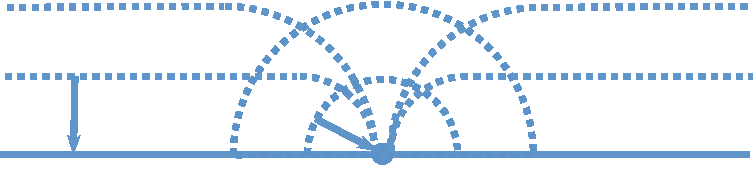
\includegraphics[width=.9\textwidth]{reg_nbhd.pdf}
	\caption{Two Sets of Tubular Neighborhoods}
	\label{fig:reg_nbhd}
\end{figure}

As the above proposition shows, control data is essential for providing Whitney stratified spaces with good neighborhoods. Not only do they endow Whitney stratified spaces with the structure of a Thom-Mather stratified space, they allow us to construct Goresky's family of lines to carry out these retractions. These retractions are instrumental to the cosheaves that we will construct in Lemma \ref{lem:strat_maps_1d} and Theorem \ref{thm:strat_maps}. There is another technical tool that we need that can only be developed in the presence of control data.

\begin{defn}\index{stratified vector field}
A \textbf{stratified vector field} $\eta$ on $(X,\{X_{\sigma}\}_{\sigma\in P_X})$ is a collection of vector fields $\{\eta_{\sigma}\}_{\sigma\in P_X}$ with one smooth vector field on each stratum.
\end{defn}

When it is meaningful to compare these vector fields, it is remarkable to note that this collection need not be continuous. Nevertheless, in the presence of control data, the flow generated by such a discontinuous vector field is continuous.

\begin{defn}
A stratified vector field $\eta$ on $X$ is said to be \textbf{controlled} by $\{T_{\sigma},\pi_{\sigma},d_{\sigma}\}$ if the following compatibility conditions are satisfied for any pair of strata $X_{\sigma}\leq X_{\tau}$:
\begin{eqnarray*}
 \eta_{\tau}(d_{\sigma,\tau}(p)) & = & 0 \\
 d(\pi_{\sigma,\tau})(\eta_{\tau}(p)) & = & \eta_{\sigma}(\pi_{\sigma,\tau}(p)) 
\end{eqnarray*}
where ever both sides of the equation are defined.
\end{defn}

\subsection{Thom Mappings}

\begin{defn}\index{stratified map!Thom mapping}
	A \textbf{Thom mapping} is a stratified map $f:(X,M)\to (Y,N)$ that satisfies \textbf{condition $a_f$} for every pair of strata $X_{\tau}\geq X_{\sigma}$: let $x_i$ be a sequence of points in $X_{\tau}$ converging to a point $p\in X_{\sigma}$. Suppose $\ker d(f|_{X_{\tau}})_{x_i}\subseteq T_{x_i} M$ converges to a plane $K\subseteq T_{p} M$, then $\ker d(f|_{X_{\sigma}})_p\subseteq K$. 
\end{defn}

\begin{figure}
	\centering
	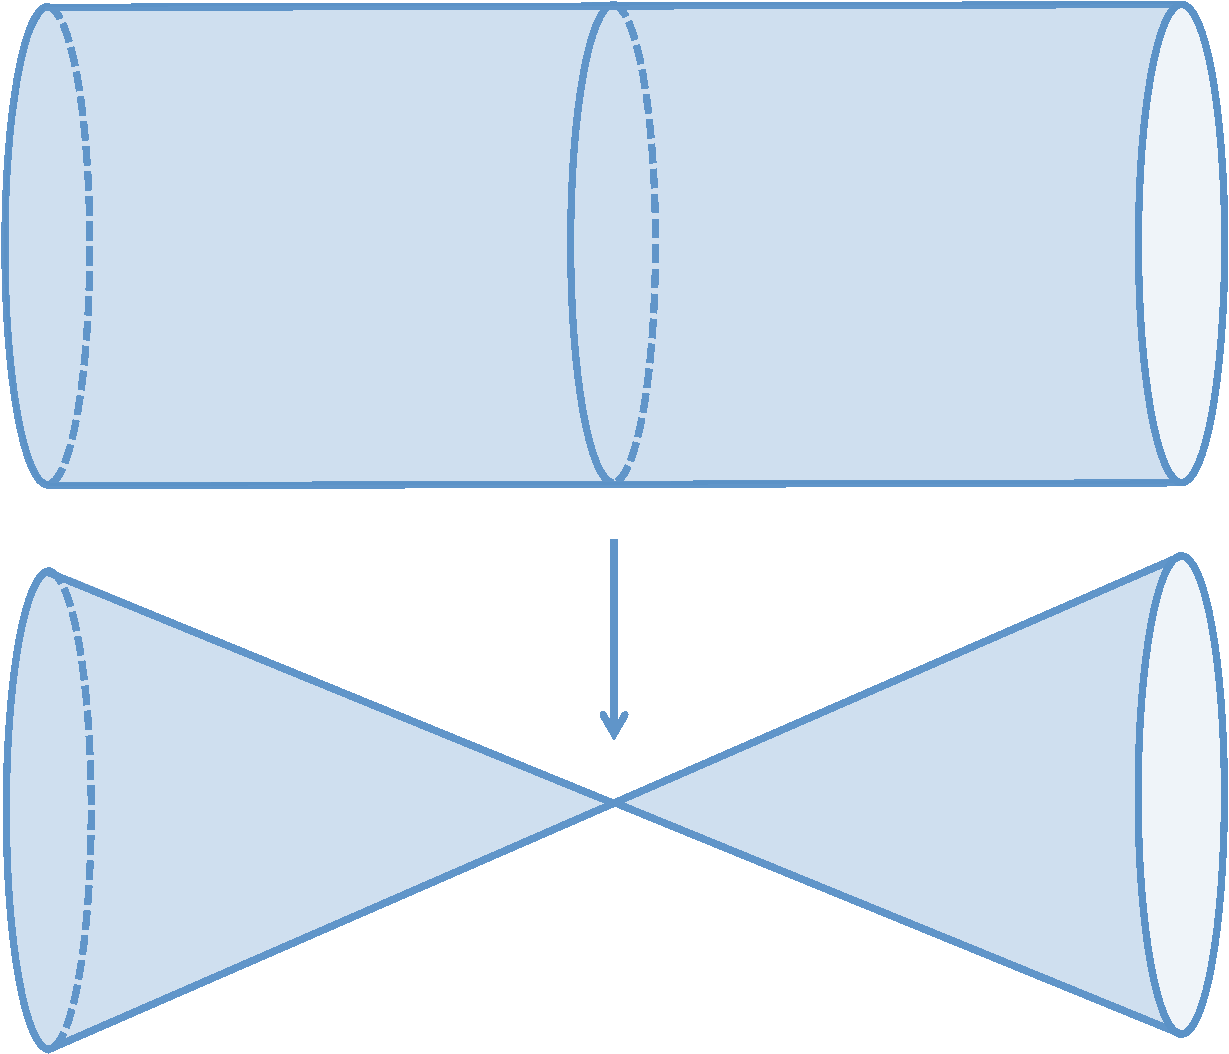
\includegraphics[width=.8\textwidth]{not_thom.pdf}
	\caption{Not a Thom Mapping}
	\label{fig:not_thom}
\end{figure}

In Figure \ref{fig:not_thom}, we have drawn an example of a mapping that is not a Thom mapping.\footnote{This example is borrowed from~\cite{lu-ctst}.} Other non-examples include the blow-up map discussed in Example \ref{ex:blowup}. Any map that is triangulable satisfies Thom's condition $a_f$ for that triangulation viewed as a stratification. It has been a long standing conjecture that every smooth Thom mapping is triangulable. Masahiro Shiota appears to have proven this conjecture in the $C^{\infty}$ case~\cite{shiota-thom}, but we have chosen not to rely on this conjecture. Instead, we only need the following proposition of Mather's (Proposition 11.3 of~\cite{mather}).

\begin{prop}\label{prop:thom_data}
	Suppose $f:X \to Y$ is a Thom mapping and a system of control data $\{T\}$ for $Y$ is given. There exists a family of tubular neighborhoods $\{T'\}$ for $X$ over $\{T\}$, which satisfies the following compatibility conditions:
	\begin{enumerate}
		\item[(a)] If $X_{\sigma}\leq X_{\tau}$, then $\pi'_{\sigma} \circ \pi'_{\tau}=\pi'_{\sigma}$ for points in $T_{\sigma}'\cap T_{\tau}'$ in $M$. Furthermore, if $f(X_{\sigma})$ and $f(X_{\tau})$ lie in the same stratum of $Y$, then $d'_{\sigma}\circ \pi'_{\tau}=d'_{\sigma}$ where both sides are defined.
		\item[(b)] If $Y_{\sigma}$ is a stratum that contains $X_{\sigma}$, then
		\[
			f(\pi'_{\sigma}(p))=\pi_{\sigma}(f(p))
		\]
		for all $p\in T'_{\sigma}\cap f^{-1}(T_{\sigma})$.
	\end{enumerate}
\end{prop}
\begin{rmk}
	The first condition is weaker than the usual definition of control data when the strata are not mapped to the same stratum. Consequently, the above notion of a \textbf{system $\{T'\}$ of control data over $\{T\}$} is not the same as two systems of control data.
\end{rmk}

Just as the notion of control data generalizes to control data over control data, controlled vector fields generalize to controlled vector fields over controlled vector fields.

\begin{defn}
Suppose $f:X\to Y$ is a Thom mapping and $\{T'\}$ is a system of control data over $\{T\}$. If $\eta=\{\eta_{\sigma}\}$ is a controlled vector field on $\{Y_{\sigma}\}$ controlled by $\{T\}$, then there exists a stratified vector field $\eta'=\{\eta'_{\sigma}\}$ on $\{X_{\sigma}\}$ satisfying the following compatibility conditions:
\begin{enumerate}
\item[(a)] For any $X_{\sigma}$ and $p\in X_{\sigma}$, we have
\[
(df|_{X_{\sigma}})(\eta'_{\sigma}(p)) = \eta_{\sigma}(f(p))
\]
where $Y_{\sigma}$ is the stratum of $Y$ that contains $f(p)$.
\item[(b)] For any $X_{\sigma}\leq X_{\tau}$, there is a neighborhood $N'_{\sigma}$ in $T'_{\sigma}$ such that for $p\in T'_{\sigma}\cap X_{\tau}$ we have
\[
d(\pi'_{\sigma,\tau})(\eta'_{\tau}(p)) = \eta'_{\sigma}(\pi'_{\sigma,\tau}(p))
\]
and if $X_{\sigma}$ and $X_{\tau}$ are carried to the same stratum of $Y$, then we have further the condition that
\[
\eta'_{\tau}(d'_{\sigma,\tau}(p)) = 0.
\]
\end{enumerate}
Thus, the notion of a \textbf{controlled vector field $\eta'$ over $\eta$} is a weaker one than a pair of controlled vector fields on $X$ and $Y$ that commute with the Thom mapping $f$.
\end{defn}

The following result, proven with help from Mark Goresky, gives a useful criterion for determining when a stratified map is a Thom mapping, so as to make the above constructions possible there. It rests on the observation that all the classical examples of stratified maps $f:X\to Y$ that aren't Thom maps require considering a pair of strata $Y_{\sigma}<Y_{\tau}$ in $Y$ whose codimension is at least two. Combinatorially, this allows us to have a pair of strata $X_{\sigma}<X_{\tau}$ in $X$ such that $\dim X_{\sigma}\cap f^{-1}(p) > \dim X_{\tau}\cap f^{-1}(x_i)$ even though $\dim X_{\sigma}<\dim X_{\tau}$. In the following lemma we show that if the codomain only has strata of codimension 1, then the map is a Thom mapping.

\begin{lem}\label{lem:thom_codim}\index{stratified map!Thom mapping}
	Suppose $f:(X,M)\to (Y,N)$ is a Whitney stratified map that is $C^1$ on the ambient manifold $M$. Let $Y'=Y_{\sigma}\cup Y_{\tau}$ be the union of two strata whose difference in dimension is one. The restricted map $f':(X',M)\to (Y',N)$ where $X':=f^{-1}(Y')$ is a Thom map.
\end{lem} 
\begin{proof}
	The proof is local, so we consider the following setup instead: Suppose $f:(X,M) \to (Y,\RR^{k+1})$ is a Whitney stratified map where $Y$ is the upper half plane in $\RR^{k+1}$, i.e. $Y:=\{(y_1,\cdots,y_{k+1})\,|\, y_{k+1}\geq 0\}$. We assume that the stratification of the map stratifies $Y$ as $Y_{\tau}:=\{y_{k+1}>0\}\cong \RR^{k+1}$ and $Y_{\sigma}:=\{y_{k+1}=0\}\cong \RR^k$. Let $X_{\sigma}$ be a stratum of $X$ that is mapped to $Y_{\sigma}$ and $X_{\tau}$ a stratum mapped to $Y_{\tau}$. Suppose $\{x_i\}$ is a sequence in $X_{\tau}$ and $\ker df|_{X_{\tau}}(x_i)=:K_i$ converges to a subspace $K_{\infty}\subseteq T_p M$ where $p\in X_{\sigma}$. We want to show that $K_p:=\ker df|_{X_{\sigma}}(p)\subseteq K_{\infty}$. By passing to a subsequence we can further assume that the tangent planes $T_{x_i} X_{\tau}=:T_i$ converges to $T_{\infty}\subseteq T_p M$. By Whitney's condition (a), $T_p X_{\sigma}\subset T_{\infty}$.
	
	Denote by $\rho_Y(y):=\pi_{k+1}(y_1,\ldots,y_{k+1})=y_{k+1}$ the ``distance from the stratum'' function on $Y$. By pre-composing with $f$, this defines a function $\rho_X(x):=\rho_Y(f(x))$. Any vector $v\in T_i$ with $d\rho_X(x_i)(v)\neq 0$ must also have $df|_{X_{\tau}}(x_i)(v)\neq 0$ since the chain rule implies that $d\rho_X(x_i)=d\rho_Y(f(x_i))\circ df|_{X_{\tau}}(x_i)$ and thus $v\notin K_i$.
	
	Let $\pi_{\sigma}:\RR^{k+1}\to Y_{\sigma}$ be the projection onto the first $k$ coordinates. The restriction of $\pi_{\sigma}$ to $Y_{\tau}$, written $\pi_{\sigma,\tau}$, is a submersion. By virtue of $\pi_{\sigma,\tau}\circ f|_{X_{\tau}}$ being a submersion, any vector $w\in T_{\pi_{\sigma}(f(x_i))} Y_{\sigma}$ has a lift $w_{f(x_i)}\in T_{f(x_i)}Y_{\tau}$ so that $w_{f(x_i)}\in \ker d\rho_Y(f(x_i))$, which in turn has a lift $\tilde{w}_i\in T_i$. Consequently, $df|_{X_{\tau}}(x_i)(\tilde{w}_i)\neq 0$ and thus $\tilde{w}_i\notin K_i$. Moreover, $\tilde{w}_i$ is orthogonal to $\nabla \rho_{X}(x_i)$ since any lift of $w$ is chosen to factor through the kernel of $d\rho_Y(f(x_i))=\pi_{k+1}$.
	
	Thus, each $T_i$ can be written as $\tilde{T}_{\pi_{\sigma}(f(x_i))} Y_{\sigma}\oplus K_i \oplus \nabla \rho_{X}(x_i)$. Since $T_p X_{\sigma}\subset T_{\infty}$ the isomorphism $T_{\infty}\cong T_p X_{\sigma}\oplus (T_p X_{\sigma})^{\perp}$ can be further refined as $T_{\infty}\cong \tilde{T}_{f(p)} Y_{\sigma} \oplus K_p \oplus (T_p X_{\sigma})^{\perp}$. We have assumed that $f$ is $C^1$ on the ambient manifold $M$ so that the lifts $\tilde{T}_{\pi_{\sigma}(f(x_i))} Y_{\sigma}$ must converge (perhaps after passing again to a subsequence) to $\tilde{T}_{f(p)} Y_{\sigma}$. Additionally, $\nabla \rho_X(x_i)$ converges to a subspace of $(T_p X_{\sigma})^{\perp}$. Finally, since $\dim X_{\sigma}< \dim X_{\tau}$, dimension constraints force $K_p\subseteq K_{\infty}$. This proves the lemma.
\end{proof}

This lemma is instrumental for our proof of Theorem \ref{thm:strat_maps}. On it's own, it has a useful corollary.

\begin{cor}
	Any stratified map $f:(X,M)\to (Y,\RR)$ that is $C^1$ on the ambient manifold is a Thom map.
\end{cor}

\subsection{Stratified Maps to the Real Line}

\begin{lem}\label{lem:strat_maps_1d}
	Any stratified map $f:X\to\RR$ defines, for each $i$, a cellular cosheaf.
\end{lem}
\begin{proof}
The map $f:X\to \RR$ defined above has as fibers the spaces $X_r$. Because it is stratifiable with finitely many strata, we have the following decomposition of the codomain:
\[
 	(-\infty,0) \leftarrow \{0\} \rightarrow (0,t_1) \leftarrow \{t_1\} \rightarrow (t_1,t_2) \leftarrow \{t_2\} \rightarrow (t_2,t_3) \cdots
\]
The points $t_i$ indicate the radii (the ``times'') where the topology of the union of the balls changes. Since the fiber $X_{t_i}:=f^{-1}(t_i)$ is a closed union of strata, proposition \ref{prop:reg_nbhd} implies (after first choosing a system of control data and then regarding $X$ as Thom-Mather stratified) that we can fix an $\epsilon>0$ such that the neighborhood $U_{t_i}(\epsilon)=\cup_{\sigma\in X_{t_i}} T_{\sigma}(\epsilon/2)$ contains $X_{t_i}$ as a weak deformation retract. Since $f$ is proper, we claim that there exists a point $s_i^-\in (t_{i-1},t_i)$ such that $X_{s_i^-}$ is contained in $U_{t_i}(\epsilon)$. Suppose for contradiction that for all $n>>0$ there exists a point $x_n\in f^{-1}([t_i-\frac{1}{n},t_i-\frac{1}{n+1}))\cap U_{t_i}(\epsilon)^c$. If this is possible, then $\{x_n\}$ defines a sequence with no convergent subsequence, which contradicts the fact that $f^{-1}([t_{i-1},t_i])$ is compact. Consequently, there exists an $n$ such that if $s_i^-:=t_i-\frac{1}{n}$, then $f^{-1}([s_i^-,t_i])\subseteq U_{t_i}(\epsilon)$. The composition of the inclusion followed by the retraction
\[
	\xymatrix{ & U_{t_i}(\epsilon) & \\ 
	X_{s_i^-} \ar@{^{(}->}[ru] & & X_{t_i} \ar@{_{(}->}[lu]_{\cong}}
\]
allows us to define maps between the homology of the typical fiber over $(t_{i-1},t_i)$ to the homology of the fiber $X_{t_i}$.
\[
	H_i(X_{s_i^-};k)\rightarrow H_i(X_{t_i};k)
\]
An analogous argument allows us to find an $s_i^+\in (t_i,t_{i+1})$ such that $X_{s_i^+}\subset U_{t_i}(\epsilon)$. We can construct a vector field on $(t_{i-1},t_i)$ that flows from the point $s_{i-1}^+$ to $s_i^-$. Lifting this vector field to a controlled one over this one, allows us to flow the fiber over $s_{i-1}^+$ to the fiber over $s_i^-$, thus realizing the homeomorphisms $X_{s_{i-1}^+}\cong X_{s_i^-}$ explicitly. For convenience, we drop the decorations and choose any point $s_i\in (t_{i-1},t_i)$ to get our modified version of the persistence module introduced in Section~\ref{subsec:pointclouds}.
\[
	\cdots \leftarrow H_i(X_{s_i};k)\rightarrow H_i(X_{t_i};k) \leftarrow H_i(X_{s_{i+1}};k)\rightarrow H_i(X_{t_{i+1}}) \leftarrow \cdots
\]
One should note that this diagram is contravariant with respect to the poset indexing the stratification of $\RR$, thus we have constructed geometrically a cellular cosheaf.
\end{proof}

\begin{cor}\index{point cloud!determines a stratified map}
	The semialgebraic function $f:X\to\RR$ in example \ref{ex:pcd} defines, for each $i$, a cellular cosheaf.
\end{cor}

Although the above construction may appear convoluted, it is geometrically natural. Instead of using the order on $\RR$ to get a diagram of vector spaces and maps, we have a diagram indexed by the pieces of a stratification of $\RR$. This new diagram is specifically adapted to the topological changes in the family $\{X_r\}$. 

In multi-dimensional persistence we imagine the need for more than one parameter to distinguish features in a point cloud. The traditional story of persistence no longer applies since $\RR^n$ for $n\geq 2$ has no natural (partial) order. In contrast, every situation where multi-dimensional persistence can be treated as a stratified map (which is effectively always), the partial order of the pieces in a stratification presents itself as a most natural candidate. 

However, the geometry of stratified spaces in more than one dimension is subtle and a poset will not always suffice. In Section \ref{subsubsec:path_cat}, we will introduce a small category (usually equivalent to a finite one) that allows us to track persistent features in a more careful way. The proof of Lemma \ref{lem:strat_maps_1d} contains the essential ideas of this more general picture. By considering certain definable paths in the parameter space, and analyzing their inverse images, which will be definable, we can try to reduce a multi-dimensional problem to a one-dimensional one. This is the high-level outline of how Theorem \ref{thm:strat_maps} associates a constructible cosheaf to a general definable map.

\section{Representations of the Entrance Path Category}
\label{subsubsec:path_cat}

Given a Whitney (or Thom-Mather) stratified space, the entrance path category looks very much like the fundamental groupoid. It has objects that are points and morphisms that are paths. However, the paths and homotopies must respect the stratification. A path may wind around in a given stratum and it may enter deeper levels of the stratification, but upon doing so, it may never return to its higher level.

\begin{figure}
	\centering
	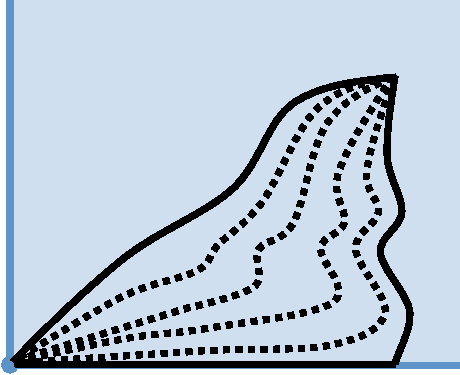
\includegraphics[width=.5\textwidth]{entr_path.pdf}
	\caption{Two Entrance Paths and a Homotopy Between Them}
	\label{fig:entr_path}
\end{figure}

\begin{defn}\index{Entr@$\Entr(X)$ entrance path category}\index{Exit@$\Exit(X)$ exit path category}
	Let $(X,\{X_{\sigma}\}_{\sigma\in P_X})$ be a Whitney (or Thom-Mather) stratified space. We define the \textbf{entrance path category} $\Entr(X,\{X_{\sigma}\})$ to be the category whose objects are points of $X$ and whose morphisms are homotopy classes of entrance paths. An \textbf{entrance path} is a path $\gamma(t)$ whose ambient dimension (the pure dimension of the containing stratum) is non-increasing with $t$. Moreover we require the homotopies $h(s,t)$ to be entrance paths for every fixed $s$. We write $\Entr(X)$ when a given stratification is understood.
	
	Opposite to the entrance path category is the \textbf{exit path category}, written $\Exit(X)$ whose objects are the same, but whose paths ascend into higher dimensional strata.
\end{defn}
\begin{rmk}[``Tame'' Homotopies]
	David Treumann's thesis~\cite{treumann-stacks}, which was written under MacPherson's direction, contains one of the first published accounts of the exit path category. However, he added an additional hypothesis that the homotopies should be ``tame,'' which he defines by saying that $h:[0,1]^2\to X$ should admit a triangulation of $[0,1]^2$ such that the interior of each simplex in the triangulation is contained in some stratum of $X$. Jon Woolf~\cite{woolf} uses a version of the exit and entrance path category based on Quinn's theory of homotopically stratified spaces and does not require Treumann's tameness assumption. Homotopically stratified spaces are more general than Whitney or Thom-Mather stratified spaces, so we may invoke some of Woolf's results. Nevertheless, Treumann's modification foreshadows our own.
\end{rmk}

\begin{defn}[Definable Entrance Path Category]\index{Entr@$\Entr(X)$ entrance path category!definable}\index{definable entrance path category}
	For a fixed analytic-geometric category $\calG$ we can consider the \textbf{definable entrance path category} to have the same objects as before, but whose morphisms are definable entrance paths, where identify entrance paths related by definable homotopies $h:I^2\to X$. There should be a triangulation of $I^2$, so that the image of every open cell is contained in some stratum of $X$. This category will be written $\Entr_{\calG}(X,\{X_{\sigma}\}).$ Dually, we have a definable exit path category $\Exit_{\calG}(X)$.
\end{defn}
\begin{rmk}
	We will not need to use the definable entrance path category until Theorem \ref{thm:strat_maps}, so one may temporarily ignore this restrictive definition. 
\end{rmk}

From the perspective of a computer, the entrance path category definition is entirely too unwieldy to be useful. Storing the points of any space we are accustomed to thinking about (circles, tori, Klein bottles, etc.) is simply too much data to consider. Fortunately, these categories are equivalent to much simpler subcategories by choosing a single point from each connected component in the stratification and passing to a skeletal subcategory.

\begin{ex}[Entrance Path Category for $S^1$]
 Now consider the circle $S^1$ stratified as a single pure stratum. The argument above shows that we can view the entrance path category of $S^1$ as equivalent to the fundamental group $\pijuan(S^1,x_0)$. This is a category with a single object $\star$ whose Hom-set corresponds to a loop for each homotopy class of path, i.e. $\Hom(\star,\star)\cong\ZZ$.
\end{ex}

\begin{ex}[Manifolds]
More generally, if the space $X$ is a manifold, stratified as a single pure stratum, then the entrance path category is equivalent to the fundamental group.
\end{ex}

If we believe MacPherson's characterization of constructible (co)sheaves, then we can reach our much sought after explanation of why cellular sheaves and cosheaves are actually sheaves and cosheaves. Part of the explanation rests on the following characterization of the entrance path category for cell complexes.

\begin{prop}[Entrance Path Category for Cell Complexes]\label{prop:ep_for_cells}\index{Entr@$\Entr(X)$ entrance path category!specializes to $\Cell(X)$}
	If $(X,\{X_{\sigma}\}_{\sigma\in P_X})$ is stratified as a cell complex, then each stratum is contractible and there is only one homotopy class of entrance paths between any two incident cells. As such
	\[
		\Entr(X)\cong\Cell(X)^{op}=P_X^{op} \qquad \mathrm{and} \qquad \Exit(X)\cong\Cell(X)=P_X.
	\]
\end{prop}

To prove this proposition, we need a better understanding of the entrance path category. To do so, we pick out a distinguished class of entrance paths.

\subsection{Homotopy Links}

\begin{defn}[Homotopy Link]\index{homotopy link}
	Suppose $X$ is a decomposed space and $X_{\sigma}\leq X_{\tau}$ are two incident pieces. The \textbf{homotopy link} of $X_{\sigma}$ in $X_{\tau}$ is defined to be the space of paths $\gamma:I\to X_{\sigma}\cup X_{\tau}$ such that $\gamma([0,1))\subset X_{\tau}$ and $\gamma(1)\in X_{\sigma}$, i.e. it is the space of paths that enter $X_{\sigma}$ at the last possible moment.
\end{defn}

We now adapt a proof of Jon Woolf's (\cite{woolf}, Lemma 3.2) to our situation. 

\begin{lem}
	Let $(X,\{X_{\sigma}\})$ be a Thom-Mather stratified space. Any entrance path is homotopic through entrance paths to an element of the homotopy link.
\end{lem}
\begin{proof}
	Suppose $\gamma:[0,1]\to X$ is an entrance path. By compactness, it can only intersect finitely many pieces in the stratification of $X$. We write $X^j$ to denote the union of all dimension $j$ pieces. For any $i\leq j$, we have that $X^i\leq X^j$. 
	
	We claim that one can show that every entrance path $\gamma$ starting in a stratum $X^k$ and ending in a stratum $X^i$ that intersects potentially every stratum in between
	\[
		X^k\geq X^{k-1} \geq \cdots \geq X^i
	\]
	is homotopic to a path $\gamma'(t)$ which sends every $t\in [0,1)$ to $X^k$ and then enters $X^i$ at the last possible moment.
	
	To define the homotopy, one focuses on pulling the path off the last stratum $X^j$ that $\gamma$ enters before entering $X^i$, i.e. there is a partition $0<t_1<\cdots < t_n< 1$ of $[0,1]$ such that $\gamma(0)\in X^k$, $\gamma([t_n,1])\subseteq X^i$ and $\gamma([t_{n-1},t_n))\subseteq X^j$. First, we show that we can pull the path off $X^i$ into $X^j$ so that it enters only at $t=1$. The schematic uses the fundamental observation that stratified spaces can be treated locally as a system of fiber bundles.

Pick a point $x_j:=\gamma(t_n-\epsilon)\in X^j$ and consider its homeomorphic image (which we call $x_j'$) in the fiber over $\gamma(t_n)$. There is a homotopy from the path $\gamma$ relative the end points $x_j=\gamma(t_n-\epsilon)$ and $\gamma(t_n)$ to the piece-wise path that is constant in the fiber, connects $x_j$ to $x_j'$, and then heads straight to $\gamma(t_n)$ while staying in the fiber over that point. By the path lifting property for fiber bundles, we can consider a lift of $\gamma([t_n,1])$ starting with $x_j'$ which ends at $x_j''$ in the fiber over $\gamma(1)$. Repeating the same argument, we can then consider a path that heads from $x''_j$ to $\gamma(1)$ while staying in the fiber. Now the path enters the stratum $X^i$ at the last possible moment.

Repeating this argument and using the conical structure of the fiber, allows us to lift the path out of the $X^j$ stratum and into higher ones. 
\end{proof}

This result allows us to take representative entrance paths that are easy to understand. Every element of the homotopy link is an entrance path, but not every entrance path is an element of the homotopy link. Moreover, it is not clear that two paths that are homotopic as entrance paths are homotopic as entrance paths (after we have moved them into the link as in the above proof). Fortunately, David Miller has recently shown this is the case~\cite{miller-popaths}. At a high level, this provides a proof of Proposition \ref{prop:ep_for_cells}, which can also be seen using easier methods.

\begin{proof}[Proof of \ref{prop:ep_for_cells}]
	Since the pieces in a cell structure on $X$ are all contractible, each cell $X_{\sigma}$ has a single path component in its homotopy link in $X_{\tau}$. Thus the skeleton of the entrance path category for a cell complex is
	\[
		\Entr(X)\cong X^{op},
	\]
which was wanted.
\end{proof}

\subsection{Van Kampen Theorem for Entrance Paths}

\begin{figure}
	\centering
	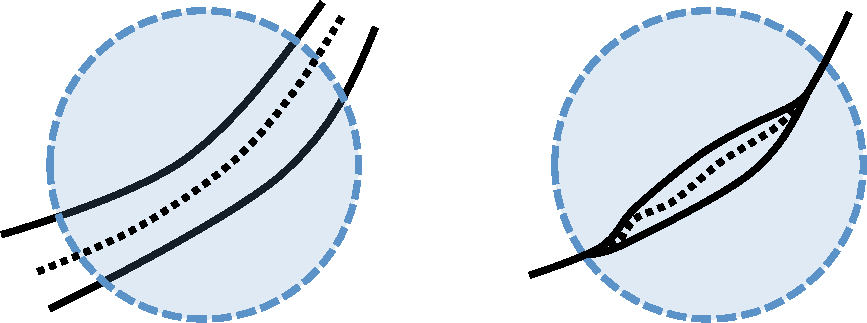
\includegraphics[width=.8\textwidth]{cover_htpy.pdf}
	\caption{Modifying a Homotopy to Stay Inside an Open Set}
	\label{fig:cover_htpy}
\end{figure}

If we can show that the entrance path category can be built up locally, then we can prove that representations of this category define cosheaves. The ability to build up locally the entrance path category is the van Kampen theorem adapted to stratified spaces. Ostensibly, David Treumann's published version of his thesis~\cite{treumann-stacks} proves the van Kampen theorem for the exit path 2-category, but the elegant inductive argument in proposition 5.9 appears to have an error.\footnote{The argument inducts on the number of triangles in a triangulation of $I^2$. The statement that the closure of the complement of a single triangle is homeomorphic to $I^2$ is not true if, for example, the triangle has two vertices on one side of the square and the third on another side.} Jacob Lurie has a proof for the $\infty$-category case~\cite{lurie-dag6}. Jon Woolf has outlined another argument~\cite{woolf-email} based on his classification of $\Set$-valued representations of the entrance path category as branched covers. The following proof, joint with Dave Lipsky, is more direct and algorithmic, but less elegant in many respects.

The main difficulty in proving the van Kampen theorem is that given a cover, a homotopy of entrance paths restricts to a free homotopy between entrance paths and not a homotopy relative endpoints; see Figure \ref{fig:cover_htpy}. In contrast to the fundamental groupoid, we cannot freely add paths to make this homotopy respect endpoints, the entrance path property must be preserved and this significantly complicates the proof. We borrow Treumann's idea of using a triangulation $T$ of $I^2$ such that $h:I^2\to X$ sends open cells of $T$ to strata of $X$. We then, after sufficient refinement, define a homeomorphism of $I^2$ that allows us to treat the triangulation as a piecewise linear one. For a piecewise linear triangulation, we outline an explicit algorithm for replacing the homotopy $h$ with a composition of homotopies preserving endpoints, each of which is supported on a triangle in $I^2$. Let us state our desired version of the van Kampen theorem and give the first step of the proof.

\begin{thm}[Van Kampen Theorem for Entrance Paths]\label{thm:vkt_ep}\index{van Kampen theorem!for Entr@$\Entr(X)$}\index{Entr@$\Entr(X)$ entrance path category!van Kampen theorem}
	If $X$ is a Whitney stratified space and $\covU=\{U_i\}$ is a cover, then
	\[
		\Entr(X)\cong \varinjlim_{I\in N(\covU)}\Entr(U_I).
	\]
	Each open set is given the induced stratification from the whole space. We assume that every homotopy $h:I^2\to X$ admits a triangulation of the domain so that for each open cell in the triangulation there is a stratum of $X$ that contains its image. Moreover, the same result holds for the definable entrance path category.
\end{thm}
\begin{proof}
	The colimit is an ordinary colimit in the category of all categories. The diagram that sends each $I\in N(\covU)$ to $\Entr(U_I)$ we will call $V$. We already know that the inclusions of the open sets $U_I\hookrightarrow X$ induce functors $\phi_I:\Entr(U_I)\to \Entr(X)$ and that these define a cocone $\phi:V\Rightarrow \Entr(X)$, i.e. a natural transformation from $V$ to the constant diagram on $N(\covU)$ with value $\Entr(X)$. Now suppose $\phi':V\Rightarrow \cat$ is another cocone. We need to check that there exists a unique map $u:\Entr(X)\to\cat$ that makes all the functors commute, i.e. $u\circ \phi_I=\phi_I'$.
	
	On objects, $u(x):=\phi_i'(x)$ for whatever open set $U_i$ contains $x$. The choice doesn't matter since if $U_j$ also contains $x$, then the functor defined on the intersection causes $\phi_i\circ \phi_{ij}(x)=\phi_j\circ\phi_{ij}(x)$. Now we must define $u(\gamma)$ for $\gamma$ an entrance path in $X$. By compactness, we can pass to a finite subcover of $\{U_i\}$ to cover the path $\gamma$. We can break up $\gamma$ into shorter paths $\gamma_{i_1},\ldots,\gamma_{i_n}$, each of which lie in some element of the cover. We define $u(\gamma):=\phi'_{i_n}(\gamma_{i_n})\circ \cdots \circ \phi'_{i_1}(\gamma_{i_1})$. We must show that this definition is invariant under homotopy to complete the proof. This is accomplished by Lemma \ref{lem:vkt_alg} together with Proposition \ref{prop:PL}.
\end{proof}
	
\begin{defn}
	Call a homotopy \textbf{$U$-elementary} if there is an interval $[a,b]\subset I$ such that $h(s,t)$ is independent of $s$ so long as $t\notin [a,b]$ and the image of $I\times [a,b]$ under $h$ is contained in $U$. See Figure \ref{fig:cover_htpy} for an illustrative cartoon.
\end{defn}

\begin{rmk}
	We will use a slightly strange way of orienting the unit square $I^2=[0,1]\times [0,1]\ni (s,t)$. The ``top edge'' is the edge where $t=0$ and the ``bottom edge'' is the edge $t=1$. We will use this language because an entrance path enters ``deeper'' levels of a stratification.
\end{rmk}


\begin{lem}\label{lem:vkt_alg}
	Let $X$ be a Whitney stratified space along with a cover $\covU$ and let $\alpha(t)$ and $\beta(t)$ be entrance paths with the same start and end points. Let $h:I^2\to X$ be a homotopy (relative endpoints) through entrance paths connecting $\alpha(t)=h(0,t)$ to $\beta(t)=h(1,t)$. If $I^2$ admits a piecewise-linear triangulation $T$ such that every open cell in $T$ is mapped to a stratum of $X$, then we may define a sequence of new homotopies $h_1,\ldots, h_n:I^2\to X$, each of which are elementary for some element of the cover, so that the composite connects $\alpha\simeq \beta$. Informally speaking, each homotopy $h_i$ will be supported on a single triangle in the barycentric subdivision of the triangulation $T$.
\end{lem}
\begin{proof}
	Since the image of $I^2$ is compact, a finite subcover of $\covU$ will do. After sufficient refinement, we can assume that each triangle in $T$ is contained in some element of the subcover. By taking the barycentric subdivision $T'$, we can refer to the vertices of any triangle in $T$ via barycentric labels $v,e,f$ depending on whether the vertex is at the barycenter of a vertex, edge or face in the original triangulation. Since each open cell in $T$ is mapped to a stratum of $X$, the triangles in $T'$ satisfy the following fundamental property: $h(\sigma_f)$, where $\sigma_f:=[v,e,f]-[v,e]$, is contained in some stratum $X_{f}$; $h(\sigma_e)$, where $[v,e]-v=\sigma_e$, is contained in $X_{e}$; $h(v)$ is contained in $X_{v}$ and $X_{f}\geq X_{e} \geq X_{v}$. We will refer to the dimension of these containing strata as the ``dimension'' of $f,v$ and $e$, respectively.
	
	By the fundamental property of triangles in $T'$ we know, for example, that the path parameterized by going from $f$ to $e$ to $v$ along the boundary of a triangle is a valid entrance path and this is homotopic through entrance paths to one that goes from $f$ directly to $v$. This is the prototypical ``move'' that we will use to define a given $h_i$ in our new homotopy between $\alpha$ to $\beta$. By reparameterizing the triangle, this move defines an elementary homotopy of entrance paths.
	
	As a preparatory step we replace the entrance path $\alpha(t):=h(0,t)$ with the path that starts at $(s,t)=(1,0)$ and goes along the top edge of the square to $(0,0)$, then to $(0,1)$ and finally to $(1,1)$. Because the homotopy is constant along the top and bottom edges, this only affects the parameterization of the path, but now our modified path and $\beta(t):=h(1,t)$ share the same endpoints in $I^2$. We will now refer to our intermediate paths $\gamma$ by a sequences of vertices in $T'$, written $w_1\cdots w_n$, which taken two at a time define edges $\gamma_i=w_{a} w_{b}$ labeled by a pair of letters $fv$ or $vf$, $fe$ or $ef$, $ev$ or $ve$. Observe that if the image of $vf$ under $h$ is a valid entrance path, then this implies that $\dim v =\dim e = \dim f$ for the triangle containing that particular edge $v_if_i$. 
	
	If an entrance path $\gamma$ ever has a vertex appear twice in its list, then this indicates a loop that must be contained in the same stratum. By virtue of the fact that $I^2$ is simply connected, the portion of the path between the repeated vertices can be homotopically reduced to the constant path via the argument used to prove the van Kampen theorem for the fundamental groupoid. We will avail ourselves of this operation, which we call the \textbf{fundamental groupoid sweep} $F$. For example, if $\gamma$ contains $\cdots e_iv_ie_i\cdots $ in its list of visited vertices, then $F(\gamma)$ will replace the portion $e_iv_ie_i$ with just $e_i$. Of course, $F^2=F$.
	
	We retain the $(s,t)$ coordinates to determine valid moves in our homotopy. We do this because, by assumption, for all $s$, $h(s,t)$ is an entrance path in $t$ and thus the dimension decreases in that direction. Now we can describe our algorithm:
	
	If $F(\gamma)=\gamma$ and $s(w_i)=s(w_j)$ for all $i\neq j$, then we are done. Otherwise, apply $F$ and starting with $\gamma_1$, ask of $\gamma_i$ if there is a triangle to the left (with respect to the induced orientation of following the path) and apply one of following rules:
	\begin{enumerate}
		\item[(1a)] If $\gamma_i=vf$ or $fv$, then replace $\gamma_i$ with $\gamma_i':=vef$ or $fev$, where $e$ belongs to the triangle to the left.
		\item[(1b)] If $\gamma_i=ev$ and $s(e)>s(v)$ or if $\gamma_i=ve$ and $s(v)>s(e)$, then $\gamma_i':=efv$ or $\gamma_i':=vfe$ where $f$ belongs to the triangle to the left.
		\item[(1c)] If $\gamma_i=fe$ and $s(f)\leq s(v)\leq s(e)$ or if $\gamma_i=ef$ and $s(e)\leq s(v) \leq s(f)$ where $v$ belongs to the triangle to the left, then $\gamma_i':=fve$ or $\gamma_i':=evf$.
	\end{enumerate}
	If none of the above apply, consider adjacent paths $\gamma_i\ast\gamma_{i+1}$ two at a time and ask if the following rule is applicable:
	\begin{enumerate}
		\item[(2)] If $\gamma_i\ast \gamma_{i+1}=fev$ or $vef$ where the interior of the triangle is kept to the left, then $(\gamma_i\ast\gamma_{i+1})'=fv$ or $vf$.
	\end{enumerate}
	After each application of a rule, one must check whether $F(\gamma)=\gamma$ and $s(w_i)=s(w_j)$ and repeat as many times as necessary. The algorithm must terminate by virtue of the fact that each step reduces the number of triangles to the left.
	
	\begin{figure}
		\centering
		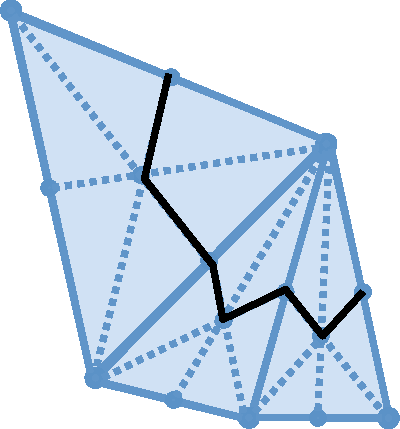
\includegraphics[width=.5\textwidth]{vkt_1c.pdf}
		\caption{Forcing Move (1c) to Apply}
		\label{fig:vkt_1c}
	\end{figure}
	
	Observe that the only way for a path $\gamma_i$ not to have a triangle to its left is if it lies on the boundary of $I^2$ and it is following the boundary clockwise. If $\gamma_i$ does not belong to the $s=1$ edge, then that contradicts the assumption that $F(\gamma)=\gamma$ as the total path must return to the point $(s,t)=(1,1)$. If the edge does lie on $s=1$, then part of the desired homotopy has been achieved and it need not be moved. If there are no triangles to the left and $F(\gamma)=\gamma$, then the algorithm has finished.
	
	The rationale for rule (1b) is that any point $p$ on the edge $ev$ determines an entrance path $h(s(p),t)$, which drops into the interior $\sigma_f$ of the triangle to the left, thus bounding the dimension of $f$ by the dimension of $e$. The rule (1c) uses similar reasoning. If $s(f)\leq s(v)\leq s(e)$ where $v$ is the triangle to the left, then the entrance path determined by $v$ $h(s(v),t)$ flows into $\sigma_f$ or $\sigma_e$ thus bounding the dimension of $e$ by the dimension of $v$. Let us now prove the correctness of the algorithm.
	
	Suppose $\gamma$ has a $vf$ of $fv$ in sequence. Since a $f$ vertex cannot belong to the boundary of $I^2$, this implies that there is a triangle to the left and that rule (1a) can be applied. Thus, to show that at least one move can be applied up until the algorithm finishes, we assume that no $vf$'s or $fv$'s appear in $\gamma$. Suppose $\gamma$ consists of only $e$'s and $v$'s. Since the start of $\gamma$ has $s(v)=1$, having $s$ non-decreasing would imply that $\gamma$ is contained in $s=1$ and the algorithm would be finished. Otherwise there is a pair such that (1b) can be applied. Now assume that our path has $e$'s, $v$'s and $f$'s, with no $fv/vf$ pairs and such that for all $ev/ve$ pairs, $s$ is increasing.
	
	Because the value of $s$ must go from $1$ back to $1$, if $s$ is not constant along $\gamma$, then there must be at least one $s$ decreasing to increasing turning point. Because $\gamma$ is piecewise linear, by turning point we mean the shortest adjacent collection of edges $\gamma_i\ast\cdots\ast\gamma_{k}$ where the $s$ value goes from strictly decreasing to strictly increasing, i.e. there is an edge along which $s$ is strictly decreasing, then potentially several edges where $s$ is constant and finally an edge which increases in $s$. To determine the ``handedness'' of these turning points we must further specify the $t$ behavior. If the turning point consists of only two edges, then we can ask if the difference in $t$ of the first and last vertex is positive or negative. If the turning point has at least one constant $s$ value edge, then we can use the difference in $t$ along the edge to determine if the turning point is $t$ positive or $t$ negative.
	
	Suppose we have a $t$ negative $s$ decreasing-to-increasing turning point. If the minimal $s$ value is obtained on this turning point, then since $t$ must go from $0$ to $1$, we can conclude that the path must intersect itself at some point, contradicting the assumption that $F(\gamma)=\gamma$. To avoid self-intersection, there must be at least one $t$ positive turning point. Since there are no decreasing $ev/ve$ pairs, the decreasing edge must be either $ef$ or $fe$. If the next term is a $v$, then either rule (1a) or (2) would have to apply, respectively. Thus, we can conclude that the next term is either an $f$ or an $e$. Inducting on the length of the $s$ constant portion of the turning point and using the fact that $f,e$ and $v$ cannot be collinear, we can show so long as rules (1a), (1b) or (2) cannot be applied, that the $s$ increasing edge has to be an $fe/ef$ edge. Consequently the last two edges in such a turning point is either $fef$ or $efe$.
	
	Now we visit the last $t$ positive $s$ decreasing-to-increasing turning point. Since the reasoning is so similar, assume that the last two edges are $efe$. We aim to show that if no other rules are applicable, then the rule (1c) must be applicable for some $ef/fe$ edge. Let us refer to the vertices in the original triangulation $T$ containing these barycenters as $v_1,v_2$ and $v_3$, whose $s$ coordinates are $s_1,s_2$ and $s_3$ respectively. Since all the vertices cannot be collinear, we let $s_2$ have the largest $s$ value. The vertex $f$ is the centroid of $\{v_1,v_2,v_3\}\subset I^2$, the first $e=e_{12}$ is the centroid of $\{v_1,v_2\}$ and the next $e=e_{23}$ is the centroid of $\{v_2,v_3\}$. By assumption $1/3(s_1+s_2+s_3)=s(f)< s(e_{23})=1/2(s_2+s_3)$, thus if the next vertex visited is $v_3$, then we can apply rule (1b) to $e_{23}v_3$. If the next vertex visited is $v_2$, then we can apply rule (2). Thus, we must assume that the next vertex is $f'=1/3(v_2+v_3+v_4)$. Now we reason on $e_{23}f'$. The next vertex cannot be a $v$, otherwise (1a) could be applied. If the next edge visited is $e_{34}$, then there are two possibilities. Either $s(e_{34})< s(f')$, which would contradict the fact that we are at the last $t$ positive turning point, or $s(f')\leq s(e_{34})$, which would imply that $2s_2\leq s_3+s_4$, but this would imply that $s_2=s(v_2)\leq s(f')$ and consequently rule (1c) would apply. Thus, assuming $s(e_{34})<s(f')$, we must remain in the link of $v_2$ and proceed to $e_{24}$. Repeating inductively, and using the fact that there are only finitely many triangles, there must be a point where rule (1c) is applicable; see Figure \ref{fig:vkt_1c}. This completes the proof.
\end{proof}

Now we must select out a class of triangulations of the unit square $I^2$ that can be deformed in an entrance-path preserving way to a PL triangulation.

\begin{prop}\label{prop:PL}
	Suppose that a (definable) triangulation $\varphi:|K|\to I^2$ by a finite simplicial complex is $C^2$ when restricted to the edges of $|K|$. There is a (definable) homeomorphism $g$ of $I^2$ so that after suitable refinement, the triangulation is piecewise-linear.
\end{prop}
\begin{proof}
	The strategy of the proof is to add additional vertices $\{w_i\}$ to the image $\varphi(e)$ of each edge in $I^2$ so that the line segment connecting any two adjacent vertices $w_0,w_1$ is to one side of the curve $\varphi(e)$ between $s(w_0)$ and $s(w_1)$. We will then locally scale the $t$ value in such a way as to push that part of $\varphi(e)$ to the line segment.
	
	To add in these vertices in a principled way, we first consider the critical set of the $s$ value of $\varphi(e)$ for every edge $e$ in $|K|$. We remove the entire critical set from $e$. If the critical set contains an interval, then we know that portion of the edge is already linear and need not consider it. Now we use the implicit function theorem to write the remainder of the edge $\varphi(e)-\{ds|_{\varphi(e)}=0\}$ as a function of $s$. For each of these functions we find the critical set of its first derivative (``inflection points'') and remove these as well. What is remaining of $\varphi(e)$ is a collection of open concave and convex arcs, each of which have boundary points $w_i,w_{i+1}$ in the various critical sets we have removed. Write $\ell_i(s)$ for the equation of the $t$ coordinate of the line connecting $w_i$ to $w_{i+1}$, i.e. the graph of the line is $(s,\ell_i(s))$. We also write the portion of $\varphi(e)$ between $w_i$ and $w_{i+1}$ as $\varphi_i(s)$.
	
	Possibly after further removal of points, we assume that each arc $\varphi_i(s)$ has a tubular neighborhood $T_i$ that contains $\ell_i(s)$ and each of these neighborhoods are pairwise disjoint. We are now going to define a homeomorphism that is the identity outside of $T_i$. To do so we need one more pair of functions.	
	\[
		\begin{array}{r c l} 
			\mu_{\pm}(x)=x & \mathrm{if} & |x|\geq 1 \\[\medskipamount]
						\mu_{\pm}(x)=2x\pm 1 & \mathrm{if} & -1 \leq x\leq \frac{-1}{2} \\[\medskipamount]
						\mu_{\pm}(x)=\frac{2}{3}x\pm \frac{1}{3} & \mathrm{if} & \frac{-1}{2} \leq 1
		\end{array}
	\]
	Now we can define a homeomorphism $g_i$ on $T_i$ using $+$ if the function $\varphi_i(s)$ is concave and $-$ if the function $\varphi_i(s)$ is convex.
	\[
		g_i(s,t):=(s,2\cdot|\varphi_i(s)-\ell_i(s)|\cdot\mu_{\pm}(\frac{t-\ell_i(s)}{2|\varphi_i(s)-\ell_i(s)|})+\ell_i(s))
	\]
	Since the domains of each $T_i$ are disjoint we can define the homeomorphism $g$ to be $g_i$ when in $T_i$ and the identity otherwise. This straightens each of the $\varphi_i(s)$. The portions of $\varphi(e)$ removed are already piecewise-linear. This makes each $g\circ \varphi(\bar{\sigma})$ into a piecewise-linear polyhedron, the interior of which is mapped via $h$ to a single stratum of $X$. By adding edges and vertices, we can refine the stratification of $g\circ \varphi(\bar{\sigma})$ to be a piece-wise linear triangulation.
\end{proof}	

\subsection{The Equivalence}
\label{subsec:equivalence_cosheaves}

We will break our proof of MacPherson's characterization into two parts. The first shows that any representation defines a constructible cosheaf. The second shows that any constructible cosheaf defines a representation of the entrance path category.

\begin{thm}[Representations are Cosheaves]\index{Entr@$\Entr(X)$ entrance path category!representations are cosheaves}\index{representation!of Entr@$\Entr(X)$}
	Let $X$ be a Thom-Mather stratified space. Any representation of the entrance path category 
	\[
		\Entr(X,\{X_{\alpha}\}) \to \Vect
	\]
	defines a constructible cosheaf.
\end{thm}
\begin{proof}
	To produce a cosheaf from a representation $\hF:\Entr(X)\to\Vect$ we take colimits over the restriction of $\hF$ to the entrance path category of $U$ (with its induced stratification):
	\[
	\hF(U):= \varinjlim_{\Entr(U)} \hF|_U
	\]
	This is clearly a pre-cosheaf since if $U\hookrightarrow V$, the colimit over $\hF|_V$ defines by restriction a cocone over $\hF|_U$ and thus a unique map $\hF(U)\to\hF(V)$. We can describe more explicitly this colimit as follows:
 
	Given a point $x\in X_{\sigma}$ in a stratum of dimension $i$, there is a basis of conical neighborhoods $U_x\cong \RR^i\times C(L)$ where $L$ is the stratified fiber of the retraction map $\pi_{\sigma}$ and $C(L)$ is its open cone. For such a neighborhood, $x$ is the terminal object in $\Entr(U_x)$, thus the colimit returns the value of $\hF(x)$. Moreover, this shows that the costalks of the pre-cosheaf defined stabilize for small contractible sets containing $x$.
	
	To show this is actually a cosheaf we use the version of the van Kampen theorem adapted to the entrance path category just proved in Theorem \ref{thm:vkt_ep}:
	\[
		\varinjlim_{I\in N(\covU)} \Entr(U_I) \cong \Entr(X)
	\]
	As a consequence of colimits commuting with colimits we get that for a representation of the entrance path category $\hF$
	\[
		 \varinjlim_{I\in N(\covU)} \hF(U_I):=\varinjlim_{I\in N(\covU)} \varinjlim_{\Entr(U_I)} \hF|_{U_I} \cong  \varinjlim_{\Entr(U_I)} \varinjlim_{I\in N(\covU)} \hF|_{U_I} \cong \varinjlim_{\Entr(U)} \hF|_U.
	\]
	This establishes the cosheaf axiom.
\end{proof}

\begin{thm}[Representations of the Entrance Path Category]\index{cosheaf!constructible!is representation of entr@$\Entr(X)$}
	Every cosheaf $\hF$ with finite-dimensional costalks that is constructible with respect to a Thom-Mather stratification of $X$ determines a representation of the entrance path category.
	\[
		\Entr(X,\{X_{\alpha}\}) \to \vect
	\]
\end{thm}
\begin{proof}
	If $X$ is a Thom-Mather stratified space, then we know that every point $x\in X_{\sigma}$ in a stratum of dimension $i$ has a neighborhood $U_x\cong \RR^i\times C(L)$, where $L$ is the fiber of $\pi_{\sigma}$, and $C(L)$ is the open cone. Now suppose $\hF$ is a constructible cosheaf, which we assume has finite-dimensional costalks. We claim that for $U_x$ suitably small we can show that
	\[
		\hF_x\cong \hF(U_x).
	\]
	This is not so easy to see and a proof would require substantial more development of cosheaf theory. Heuristically, if the value of $\hF$ on a sequence of conical neighborhoods never stabilized then this would contradict the constancy of the cosheaf on sets of the form $U_x\cap X_{\tau}$. For a rigorous proof, one dualizes a constructible cosheaf to a constructible sheaf by post-composing with $\Hom_{\vect}(-,k)$, which is an equivalence, and we can apply the proof for constructible sheaves found on p. 84 of~\cite{gm-ih2}. 
	
	Consequently, if $y\in U_x\cap X_{\tau}$ is a point in a nearby stratum, then there is an analogous neighborhood $U_y$ contained in $U_x$. Repeating the same argument, we can then use the maps present in a cosheaf to define a map from the costalk at $y$ to the costalk at $x$:
	\[
		\xymatrix{\hF_x \ar[r]^-{\cong} & \hF(U_x) & \ar[l] \hF(U_y) & \ar[l]_-{\cong} \hF_y}
	\]
	Recall that the restriction of a constructible cosheaf to any stratum defines a locally constant cosheaf. For arbitrary points $y'$ in the stratum $X_{\tau}$ we can consider a path $y'\rightsquigarrow y$ and use Theorem \ref{thm:lc_sheaf_rep} to define a map from $\hF_{y'}$ to $\hF_{y}$. Postcomposing with the above map defines the map $\hF_{y'}\to \hF_{x}$. This explains why constructible cosheaves map naturally define ways of specializing a costalk over one stratum to a costalk in its frontier.

	To show homotopy invariance, we appeal to the van Kampen Theorem \ref{thm:vkt_ep} to reduce the argument to elementary homotopies of a particular form. Assume $\alpha(t)$ goes from $z\in X_{\lambda}$ directly to $x\in X_{\sigma}$ and that $\beta(t)$ goes from $z$ to $y$ and then $x$. Since restriction to any stratum defines a locally constant cosheaf, we can appeal to the homotopy invariance of Theorem \ref{thm:lc_sheaf_rep} to position these paths and points to be inside $U_x$ and so that $U_x\supset U_y\supset U_z$. By choosing a similar set of isomorphisms, we get two commutative diagrams, which followed along the top edge corresponds to the action of $\alpha(t)$ and followed along the bottom edges corresponds to $\beta(t)$.
 	\[
		\xymatrix{\hF(U_z) \ar[rr] \ar[rd] & & \hF(U_x) \\ & \hF(U_y) \ar[ru] &} \qquad \qquad \qquad 
		\xymatrix{\hF_{z} \ar[rr] \ar[rd] & & \hF_{y} \\ & \hF_{x} \ar[ru] &}
	\]
\end{proof}

\subsection{Representations from Stratified Maps}

We want to show that stratified maps induce representations of the entrance path category, which, by the first part of our equivalence, defines a constructible cosheaf.

\begin{thm}[Cosheaves from Stratified Maps]\label{thm:strat_maps}\index{cosheaf!constructible!from a definable map}\index{stratified map!determines constructible cosheaves}\index{representation!of entr@$\Entr(X)$! from a stratified map}
	Fix an analytic-geometric category $\calG$. If $Y$ is a closed set in $\calG(N)$ and $f:(Y,N)\to (X,M)$ is a $C^1$ proper definable map, then for each $i$, the assignment
	\[
		x\in X \rightsquigarrow H_i(f^{-1}(x);k)
 	\]
defines a representation of the definable entrance path category of $X$, where the stratification is gotten by the stratification induced by $f$.
\end{thm}
\begin{proof}
	Let $\gamma:I\to X$ be a definable map that satisfies the entrance path condition, i.e. as $t$ increases the dimension of the ambient stratum is non-increasing. Thus $\gamma(0)$ is in a stratum of dimension greater than or equal to $\gamma(1)$. By Lemma \ref{lem:def_pb}, we know that the pullback $Y_{\gamma}:=I\times_X Y$ is definable, as is the pullback of $f$ along $\gamma$, written $\gamma^*f$. Since definable sets can be Whitney stratified, $Y_{\gamma}$ admits a system of control data, and may be regarded as a Thom-Mather stratified space.
	
	The argument from Lemma \ref{lem:strat_maps_1d} provides us with the prototype for getting a diagram of spaces for every path. We will repeat it here for convenience and make any necessary modifications. By definable triviality (4.11 of~\cite{vdd-geocat}), there exists a finite partition of $[0,1]$ such that over each interval the inverse image is homeomorphic to the product:
	\[
		\xymatrix{f^{-1}((t_i,t_{i+1})) \ar[rr]^{\cong} \ar[rd]_f & & F\times (t_i,t_{i+1}) \ar[ld] \\ & (t_i,t_{i+1}) &}
	\]
	By properness we can, for any fixed $\epsilon>0$, find an $s_i^+$ such that $f^{-1}([t_i,s_i^+])$ is contained in $U_{i}(\epsilon):=\cup T_{\sigma}(\epsilon/2)$ for $Y_{\sigma}\subseteq f^{-1}(t_{i}):=Y_{i}$. The retraction we constructed in Proposition \ref{prop:reg_nbhd} gives a retraction map $r_i^+:=H(p,0)$ from $U_{i}(\epsilon)\to Y_{i}$. This allows us to define a map on fibers
	\[
		f^{-1}(s_i^+) \hookrightarrow U_{i}(\epsilon) \to Y_{i}.
	\]
	Applying some homology functor $H_n(-;k)$ defines the representation locally on the path. Of course, we must show that this representation is independent of the point $s_i$ taken. If $s_i^{+'}\in [t_{i},s_i^+]$ is another point, then the composition of the trivialization with the retraction witnesses the homotopy between these two choices.
	\[
	 F\times [s_i^{+'},s_i^+]\cong f^{-1}([s_i^{+'},s_i^{+}])\hookrightarrow U_{i}(\epsilon) \to Y_{i}
	\]
	Similarly, one can find a point $s_{i+1}^-$ so that it's fiber is contained in $U_{i+1}(\epsilon)$ and the retraction $r_{i+1}^-$ defines a map from that fiber to the fiber $Y_{i+1}=f^{-1}(t_{i+1})$. 
By Thom's first isotopy lemma there is a homeomorphism $\varphi_{i+1,i}$ taking the fiber over $s_{i}^+$ to the fiber over $s_{i+1}^-$. This homeomorphism is gotten by constructing a vector field that flows from $s_i^+$ to $s_{i+1}^-$ and lifting it to a controlled vector field on $f^{-1}((t_i,t_{i+1}))$ via Proposition 9.1 of~\cite{mather}. 
	Finally, one must observe that the filtration of $X$ by strata of a given dimension or less, the restriction of $\gamma$ to the half-open interval $[t_i,t_{i+1})$ is contained inside a single stratum of $X$ and thus the retraction $r_i^+$ induces a homotopy equivalence between the fiber over $s_i^+$ and the fiber over $t_i$. Applying our homology functor to the following composition defines the total action associated to this path:
	\[
		\cdots (r_{i+1})_*^-\circ (\varphi_{i+1,i})_* \circ (r_{i}^+)_*^{-1} \cdots
	\]

	\begin{figure}
		\centering
		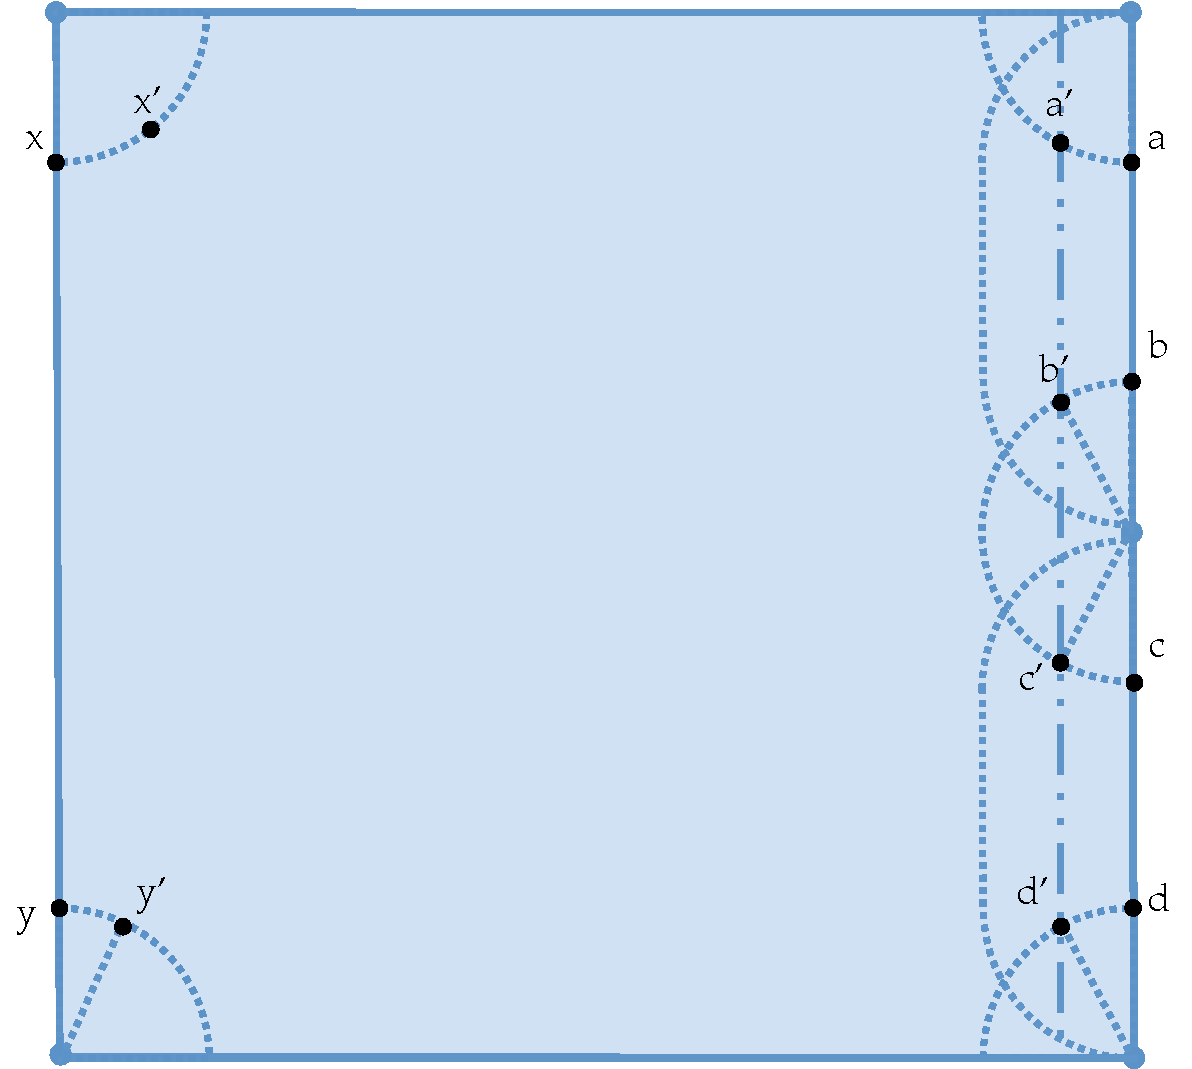
\includegraphics[width=.8\textwidth]{strat_maps_htpy.pdf}
		\caption{Argument for Homotopy Invariance}
		\label{fig:strat_maps_htpy}
	\end{figure}
	
	It remains to be seen that this map is invariant under definable homotopies of entrance paths. Suppose $h:I\times I\to X$ is a definable homotopy. Again, the pullback $Y_h:=I^2\times_X Y$ is definable, as is the map $h^*f$, and both can be stratified. Thus, we have reduced everything to considering a stratified map to the square $I^2$. By the van Kampen Theorem \ref{thm:vkt_ep}, it suffices to check homotopy invariance on an elementary homotopy, such as the one depicted in Figure \ref{fig:entr_path}. Let us assume that $h$ is a homotopy between an entrance path $\alpha(t)=h(0,t)$, which goes from a stratum $X_{\lambda}$ and enters a stratum $X_{\sigma}$ at the last possible moment $t=1$, and an entrance path $\beta(t)=h(1,t)$, which enters $X_{\tau}$ at $t=1/2$ and then goes to $X_{\sigma}$ at $t=1$. Moreover, we assume that $h$ takes the complement of $\{t=1\}\cup \{(1,t)\,|\, t\geq 1/2\}$ to the stratum $X_{\lambda}$. This guarantees that the fibers over $x,x',y,y',a,a',b,b',c'$ and $d'$ in Figure \ref{fig:strat_maps_htpy} can all be identified.

Let ${T}$ be a system of control data for $Y_h$, obtained in a specific way. By restricting to the strata over $s=0$ and $s=1$ respectively, we get control data for $Y_{s=0}$ and $Y_{s=1}$, both of which are inside $I^2\times_X Y\subset \RR^2\times N$. The spaces $Y_{s=0}$ and $Y_{s=1}$ can be identified with the inclusions of $Y_{\alpha}$ or $Y_{\beta}$, which are contained in $\RR\times N$. The manner in which Mather constructs control data in Proposition 7.1 of~\cite{mather} can be used to extend the control data for $Y_{\alpha}$ and $Y_{\beta}$ to control data for $Y_{s=0}$ and $Y_{s=1}$ inside $\RR^2\times N$ respectively. This is how we obtain those tubular neighborhoods in $\{T\}$ and the rest can be constructed to be compatible with those. This allows us to use the control data ${T}$ to meaningfully compare the construction above for $\alpha(t)$ and $\beta(t)$.
 	
	We can describe the maps associated to $\alpha(t)$ and $\beta(t)$ as follows: By properness, we assume the fiber over $x$ is contained in a regular neighborhood, which retracts via $r_x$ to the fiber over $(0,0)$. There is a homeomorphism $\varphi_{y,x}$ from the fiber over $x$ to the fiber over $y$. Finally, we can assume that the fiber over $y$ retracts via $r_y$ to the fiber over $(0,1)$. Thus the action associated to $\alpha(t)$ is the map
	\[
		(r_y)_*\circ(\varphi_{y,x})_*\circ (r_x)^{-1}_*:H_n(Y_{(0,0)})\to H_n(Y_{(0,1)})
	\]
	where we have implicitly pre-composed $r_x$ with the inclusion of the fiber.

	For $\beta(t)$, the action is similar:
	\[
		(r_d)_*\circ (\varphi_{d,c})_*\circ (r_c)_*^{-1}\circ (r_b)_*\circ (\varphi_{b,a})_*\circ (r_a)^{-1}_*: H_n(Y_{(1,0)})\to H_n(Y_{(1,1/2)}) \to H_n(Y_{(1,1)})
	\] 
	
	The strategy of the proof is to pick a path $\gamma(t)$ that interpolates $\alpha(t)$ and $\beta(t)$ and show that the associated map on homology agrees with both $\alpha(t)$ and $\beta(t)$. This path is indicated by the dotted-and-dashed line passing through $a',b',c'$ and $d'$ in Figure \ref{fig:strat_maps_htpy}. The representation associated to $\gamma(t)$ is
	\[
		(r_{1})_*\circ (\varphi_{d',c'})_*\circ (i_{c'})_*^{-1} \circ (i_{b'})_* \circ (\varphi_{b',a'})_* \circ (r_{0})^{-1}_*.
	\]
        Here the maps $i_{b'}$ and $i_{c'}$ denote the inclusion of $Y_{b'}$ and $Y_{c'}$ into the inverse image of the interval $[b',c']$. The action on homology of $(i_{c'})_*^{-1} \circ (i_{b'})_*$ agrees with an analogously constructed homeomorphism $\varphi_{c',b'}$, but we will find it easier to equate the map associated to $\beta(t)$ and $\gamma(t)$ as written above.

        Because the control data $\{T\}$ extends the control data for $Y_{\alpha}$ and $Y_{\beta}$, the retraction map $r_a$ can be taken to be the restriction of a retraction map $r_{0}:U_{Y_{(1,0)}}(\epsilon)\to Y_{(1,0)}$ constructed in Proposition \ref{prop:reg_nbhd}. This in turn can be taken to be the restriction of the tubular projections used to define a retraction map $r_{s=1}:U_{s=1}(\epsilon)\to Y_{s=1}$. The commutation relations for control data allow us to imagine first taking the fiber $Y_{a'}$ over $a'$ and retracting to the strata over the edge $e_0:=\{(1,t)\,|\, 0<t<1/2\}$, and then retracting to the fiber over $(1,0)$. This allows us to factor $r_{0}$ as
\[
r_{0}=r_{a}\circ r_{e_0},
\]
but the image of $Y_{a'}$ under $r_{e_0}$ may not be contained in $Y_{a}$ or any single fiber. This would be true if, for example, the control data defining the retraction to $Y_{e_0}$ satisfied
\[
\pi_{e_0}(f(p))=f(\pi_{\sigma}(p))
\]
for each stratum $Y_{\sigma}$ that $f$ carried to $e_0$, but in general it does not. This is what necessitates the use of the Thom properties given by Lemma \ref{lem:thom_codim} and property (b) of Proposition \ref{prop:thom_data}.

By Lemma \ref{lem:thom_codim}, we know that restricting the codomain to the complement of the vertices, the mapping $h^*f$ is a Thom mapping. Consequently, if we pick a tubular neighborhood $T_{e_{0}}$ for the edge $e_0:=\{(1,t)\,|\, 0<t<1/2\}$, there exists a system of control data $\{T'\}$ over $T_{e_0}$ and the interior of $I^2$ by Proposition \ref{prop:thom_data}. If we restrict to those tubular neighborhoods coming from strata in $Y_{e_0}$, then property (a) of Proposition \ref{prop:thom_data} implies that this restricted collection of tubular neighborhoods defines actual control data for $Y_{e_0}$, which we call $\{T'\}_{Y_{e_0}}$. A priori, the analogous restriction of $\{T\}$ to $Y_{e_0}$ defines a different system of control data. However, by Mather's uniqueness result,\footnote{Mather mentions at the bottom of page 492 of~\cite{mather} that any Whitney stratified subset $Z$ of a manifold $M$ has a unique, up to isomorphism, structure as a Thom-Mather stratified set. This is not explicitly proved, but it follows from Mather's Corollary 10.3 as explained by Goresky: Suppose $Z$ is given two different structures of control data $\{T\}$ and $\{T'\}$. If we consider $Z\times\RR$ as a Whitney stratified subset of $M\times \RR$, then $\{T\}$ and $\{T'\}$ can be extended to control data on $Z\times(-\epsilon,\epsilon)$ and $Z\times (1-\epsilon,1+\epsilon)$, respectively. Then, using the proof of prop. 7.1, one can find control data on all of $Z\times\RR$ that agrees with the $\epsilon$ extensions of $\{T\}$ and $\{T'\}$. This space, now viewed as a Thom-Mather stratified set, is then isomorphic via Corollary 10.3 to the set where just $Z\times\RR$ is given the extension of just the control data $\{T\}$.} there is a homeomorphism $\psi_{e_0}$ of $Y_{e_0}$ that takes $\{T'\}_{Y_{e_0}}$ to $\{T\}_{Y_{e_0}}$. This implies that if $Y_{\sigma}$ is a stratum that is mapped to $(1,0)$ and $Y_{\tau}$ is mapped to $e_0$, then
\[
\pi_{\sigma}=\pi_{\sigma}\circ\psi_{e_0}\circ \pi_{\tau'} \qquad \mathrm{since} \qquad \pi_{\tau}=\psi_{e_0}\circ \pi_{\sigma'}
\]
By repeating the construction of a retraction outlined in Proposition \ref{prop:reg_nbhd}, but using the control data $\{T'\}_{Y_{e_0}}$ instead to construct the family of lines, we get a map $r'_{e_0}$ that carries the fiber over $a'$ to the fiber over $a$. Post-composing $r'_{e_0}$ with $\psi_{e_0}$ gives the equality $r_{e_0}=\psi_{e_0}\circ r'_{e_0}$. This construction gives the left most triangle in the following commutative diagram:
\[
\xymatrix{Y_{(1,0)} & \ar[l]_{r_a \psi_{e_0}} Y_a \ar[r]^{\varphi_{b,a}} & Y_b \ar[r]^{r_b\psi_{e_0}} & Y_{(1,1/2)} & \ar[l]_{r_c\psi_{e_1}} Y_c \ar[r]^{\varphi_{d,c}} & Y_d \ar[r]^{r_d\psi_{e_1}} & Y_{(1,1)} \\
& \ar[lu]^{r_{0}} Y_{a'} \ar[u]_{r'_{e_0}} \ar[r]_{\varphi_{b',a'}} & Y_{b'} \ar[u]^{r'_{e_0}} \ar[ur]_{r_{1/2}} \ar[r]_{i_{b'}} & Y_{[b',c']} \ar[u]_{r_{1/2}} & \ar[l]^{i_{c'}} \ar[lu]_{r_{1/2}} Y_{c'} \ar[u]_{r'_{e_1}} \ar[r]_{\varphi_{d',c'}} & Y_{d'} \ar[u]^{r'_{e_1}} \ar[ur]_{r_{1}} & }
\]

Now we explain the other maps in this diagram. The homeomorphisms $\varphi_{b,a}$ and $\varphi_{b',a'}$ are constructed by taking a controlled vector field $\{\eta_f,\eta_{e_0},\eta_{e_1}\}$ in $I^2$ minus the vertices using the control data $\{T'\}$ over $\{T_f,T_{e_0},T_{e_1}\}$. Since $d\pi_{e_0}(\eta_f(s,t))=\eta_{e_0}(\pi_{e_0}(s,t))$ the controlled vector field over this one commutes with $f$ and gives
\[
\varphi_{b,a}\circ r_{e'_0}=r_{e_0'}\circ\varphi_{b',a'}.
\]

Again, the commutation relations in Proposition \ref{prop:reg_nbhd} allows us to, using the control data $\{T\}$ to factor $r_{1/2}=r_{b}\circ r_{e_0}$. However, the uniqueness theorem tells us that $r_{e_0}=\psi_{e_o}\circ r'_{e_0}$ where $\psi_{e_0}$. A simple diagram chase now completes the argument. Comparing the maps associated to $\alpha(t)$ and $\gamma(t)$ is much simpler and uses the same ideas. We leave it to the reader. 
\end{proof}

\begin{rmk}[Alternative Idea for a Proof]
	An alternative approach makes use of the properties of o-minimal structures. The generic triviality theorem 4.11 of~\cite{vdd-geocat} guarantees that we have a definable trivialization of the map over $(0,1)$.
	\[
		\xymatrix{f^{-1}(\gamma((0,1))) \ar[rr]^{\cong}_h \ar[rd]_{\gamma^*f} & & F\times (0,1) \ar[ld] \\ & (0,1) & }
	\]
	For each point $x$ in the fiber $F$, we get a lift $\{x\}\times (0,1)$ of the open interval. Applying the inverse homeomorphism, $h^{-1}(\{x\}\times (0,1))$ defines a definable path $\alpha_x:(0,1)\to f^{-1}(\gamma([0,1]))$. 
	
	M\'ario Edmundo and Luca Prelli, in their recent note~\cite{edmundo-six} reworking the six basic Grothendieck operations for sheaves in the o-minimal setting, have given a tantalizing reformulation of what characterizes a definable proper map. They use an idea of Ya'acov Peterzil and Charles Steinhorn~\cite{peterzil-cpt} that shows that being definably compact (equivalently, closed and bounded) is equivalent to being able to to complete curves. A map $f:Y\to X$ is definably proper if for every definable curve $\alpha:(0,1)\to Y$ and every definable map $[0,1]\to X$ there is at least one way to complete the diagram:
	\[
		\xymatrix{ (0,1) \ar[r]^{\alpha} \ar[d] & Y \ar[d]^{f} \\
		[0,1] \ar[r] \ar[ur]_{\bar{\alpha}} & X}
	\]
	If one assumes all the maps are continuous as well as definable then the completion in the diagram above is unique.\footnote{One of the unusual features of o-minimal topology is that definable maps need not always be continuous, thus the added hypothesis. Even discontinuous maps can have triangulable graphs.}
	
	In our situation, the hypotheses guarantee that for each point $x\in F$, we can complete the curve $\alpha_x:(0,1)\to I\times_X Y$ to a curve $\bar{\alpha}_x:[0,1]$. By associating endpoints over $0$ to endpoints over $1$ we define a set-theoretic map $g:f^{-1}(\gamma(0))\to f^{-1}(\gamma(1))$. The hard work is showing that this map $g$ is continuous and is invariant under homotopy.
\end{rmk}
